\documentclass[12pt]{gsis}  % 12pt font required by GSIS
\usepackage{epstopdf}
\usepackage{graphicx,subfigure}
\usepackage{hyperref,caption}
\usepackage[para,online,flushleft]{threeparttable}
\usepackage{multirow,booktabs}
\usepackage{geometry}
\usepackage{natbib}
\usepackage{longtable}
\usepackage{url}
\usepackage{array}
\usepackage{float}
\bibpunct[, ]{(}{)}{;}{a}{}{,}
\renewcommand\bibfont{\fontsize{10}{12}\selectfont}

\begin{document}

\copyrightyear{2026}

\title{Grounded Geo-LLM Workflow Contracts for Reliable GIS Copilots: A Reproducible Benchmark Across Local Open-Source Models}

\author[a]{Nguyen The-Vinh\thanks{CONTACT Nguyen The-Vinh. Email: vinhnt@ictu.edu.vn}}
\author[a]{Nguyen Kim-Son}
\affil[a]{Department of Software Engineering, Faculty of Information Technology, Thai Nguyen University of Information and Communication Technology, Thai Nguyen University, Thai Nguyen City, Vietnam}

\keywords{GIS copilot; large language models; GeoAI; workflow specification; geospatial validation}

\Abstract{Large language models are increasingly used as natural-language interfaces to geographic information systems (GIS), but free-form code generation obscures whether failures arise from wrong spatial plans, hallucinated data, coordinate-reference-system (CRS) errors, software syntax, or weak map outputs. This paper introduces a workflow-contract benchmark for Geo-LLM GIS copilots. Instead of asking models to generate code directly, the benchmark requires structured JSON specifications that bind user intent to known layers, fields, spatial operations, CRS assumptions, validation checks, and output artifacts. Twelve local Ollama models are evaluated on 30 GIS workflow tasks under task-only, metadata-grounded, and GeoGuard-style validation prompts, yielding 1080 attempted specifications across buffer, overlay, point-count, raster-clip, zonal-statistics, and choropleth-export families. Metadata grounding is the dominant anti-hallucination intervention: mean data validity rises from 0.053 to 0.761, weighted hallucination risk falls from 0.522 to 0.277, and plan reliability rises from 0.547 to 0.751. GeoGuard validation adds a spatially specific gain, raising mean CRS planning from 0.674 to 0.774 and reducing CRS-weak cases from 89 to 39 out of 360 tasks. Full-cohort deterministic execution produces 43, 230, and 233 valid GIS artifacts for basic, grounded, and GeoGuard modes, and a 2165-case negative-control audit detects injected contract faults at rates from 0.943 to 1.000. The benchmark provides a reproducible computer-science evaluation layer for testing whether Geo-LLM systems preserve geographic meaning before code execution and map rendering.}

\newgeometry{top=20.0mm,bottom=40.0mm,left=15mm,right=15mm,headsep=8mm}
\maketitle
\restoregeometry
\newpage

\section{Introduction}

Large language models (LLMs) are increasingly positioned as natural-language interfaces to geographic information systems (GIS). For geoinformatics, the central technical question is not simply whether a model can discuss places, but whether it can be connected to spatial data, operators, validation rules, and output artifacts in a way that remains reliable across GIS workflows. A user can ask for a buffer, overlay, point-in-polygon count, raster clip, zonal statistic, or choropleth map and receive executable code in return. This interaction is attractive because GIS work combines declarative analytical intent with procedural software details. Yet GIS is not only a programming domain. Since the emergence of geographical information science, spatial computation has been understood as a discipline in which location, scale, topology, spatial dependence, measurement, and representation shape validity \citep{Goodchild_1992,Tobler_1970,Anselin_1995,Janowicz_2019}. The geoinformatics literature has treated these concerns as computer-science problems for GIS: spatial concepts can be formalized as data models, spatial analysis tasks can be cast as scalable algorithms, and GIS procedures can be evaluated as reusable computational methods \citep{Shekhar_1999_ObjectDirection,Shekhar_2003_SpatialOutliers,Yoo_2005_InRouteNN,Camelli_2012_SeamlessSurfaces}. A GIS assistant can therefore fail even when code is syntactically plausible: it may buffer in angular units, overlay layers with incompatible coordinate reference systems (CRS), invent a field, drop a derived attribute, clip a raster with an unaligned mask, or render a map whose legend and thematic field do not support the user's geographic question.

Existing LLM evaluation does not fully expose this problem. General code-generation benchmarks have established that model performance depends strongly on task structure, context, and evaluation protocol \citep{Li_2022,Xu_2022,Du_2024,Ni_2024,Jiang_2026}. Geospatial-code studies move the discussion closer to GIS by asking whether LLMs can generate geospatial code or use operator knowledge for platforms such as Google Earth Engine \citep{Hou_2025_GeoCode,Hou_2025_GEEOPs}. Recent work on autonomous GIS argues that LLMs may become decision cores that generate and execute geoprocessing workflows \citep{Li_2025_AutonomousGIS}. That vision makes the evaluation problem sharper: a code- or application-level benchmark merges several failure sources into one outcome. A failed script may reflect a wrong spatial plan, a hallucinated dataset, a library syntax error, a changed API, or a missing import. Conversely, a script can run while still producing an invalid spatial analysis or a weak cartographic artifact. This diagnostic entanglement is especially problematic for GIS because the spatial assumptions that determine analytic validity are often implicit in code.

The missing layer is an inspectable contract between a natural-language GIS request and executable code. In conventional GIS practice, analysts routinely reason about input layers, fields, CRS transformations, spatial predicates, output schemas, and map-design requirements before running an operation. These commitments resemble data and model documentation practices that make assumptions explicit \citep{Gebru2021Datasheets,Mitchell2019ModelCards}, and they align with theory-guided and constraint-aware views of scientific machine learning \citep{Karpatne_2017}. However, current LLM-GIS evaluations rarely isolate this planning contract as the unit of measurement. As a result, it remains unclear whether local open-source models fail because they cannot write Python, because they lack grounded data context, or because they cannot formulate a geospatially valid workflow plan.

This paper addresses that gap by introducing a workflow-contract benchmark for LLM-GIS copilots. Instead of asking a model to write free-form code, the benchmark asks it to return one structured JSON object that specifies the operation, input layers, parameters, output artifact, required fields, validation checks, and a short rationale. The scorer then evaluates the contract itself: parseability, operation validity, known-layer use, field validity, CRS planning, schema preservation, map-export planning, output naming, hallucination risk, and an overall plan reliability score. This design creates an earlier diagnostic layer at which metadata grounding, tool schemas, and validation rules can be tested before code generation or map rendering begins. The study therefore treats LLM-GIS reliability as a spatial-computing interface problem: a natural-language request must be transformed into an explicit, testable GIS object before it is allowed to drive software execution.

The novelty is threefold. First, the benchmark treats Geo-LLM reliability as a geospatial workflow-contract problem rather than only as a code-generation problem. Second, it operationalizes spatial and cartographic validity criteria that are central to GIS but usually absent from generic programming benchmarks: CRS strategy, layer and field grounding, schema transition, raster-vector alignment, and map-plan completeness \citep{Roth_2013,Roth_2015,Kang_2024,Munzner_2009}. Third, it evaluates local open-source models under controlled prompting regimes, making it possible to separate task-only planning from metadata-grounded planning and GeoGuard-style validation. This framing matches the computer-science-for-GIS scope of geoinformatics: the contribution is a reusable evaluation protocol, scorer, and execution gate that are applicable across multiple spatial-analysis and map-export families rather than a single GIS application case.

The experiment covers twelve locally installed Ollama models, 30 GIS workflow tasks, and three prompting modes, yielding 1080 attempted workflow specifications. The task suite spans buffer service areas, flood-zone overlay, school and hospital point-count joins, raster clipping, zonal statistics, and choropleth export. These families map directly to a core Geo-LLM concern: integrating LLMs and geospatial data for decision-support settings such as urban services, exposure analysis, environmental raster processing, and thematic communication. The paper asks four empirical questions within this introduction: how much metadata grounding reduces layer and field hallucination; whether validation rules improve CRS, schema, and execution-readiness outcomes beyond grounding alone; which task and model families remain difficult under a strict structured-output protocol; and whether passing contracts can be deterministically bound to real layers and executed into valid GIS artifacts. By answering these questions at the planning-contract and initial execution layers, the study provides a reproducible benchmark for measuring whether Geo-LLM GIS copilots preserve geographic meaning before and during downstream execution.

\section{Related Work}

\subsection{LLMs for code and workflow generation}

Modern language models can generate executable code, solve programming problems, and assist software repair, but their reliability varies with task structure, context, and evaluation protocol \citep{Li_2022,Xu_2022,Du_2024,Ni_2024,Jiang_2026}. Software-engineering work also shows that repair and validation loops can convert some failed outputs into usable artifacts, while leaving difficult semantic failures unresolved \citep{Gazzola_2019,Monperrus_2018,Le_Goues_2012}. These lessons transfer naturally to GIS, where a script must satisfy both software and spatial contracts.

This transfer is aligned with a longer geoinformatics pattern: GIS reliability improves when spatial tasks are made explicit enough to support formal reasoning, scalable implementation, and reproducible evaluation. Examples include modeling direction as a first-class spatial object for query processing \citep{Shekhar_1999_ObjectDirection}, defining spatial outliers and scalable detection algorithms \citep{Shekhar_2003_SpatialOutliers}, comparing alternative query-processing strategies for in-route nearest-neighbor search \citep{Yoo_2005_InRouteNN}, and deriving seamless triangulated surfaces for physical modeling from GIS inputs \citep{Camelli_2012_SeamlessSurfaces}. The present benchmark follows the same systems-oriented logic for Geo-LLM interfaces: it makes the intermediate GIS plan explicit so that it can be scored, compared, and executed by deterministic components.

Recent geospatial-code-generation work moves this question into GIScience directly. GeoCode-style benchmarks ask whether LLMs can answer or produce geospatial code across API and task families, while operator-knowledge approaches such as GEE-OPs improve Google Earth Engine code generation by exposing structured operation knowledge \citep{Hou_2025_GeoCode,Hou_2025_GEEOPs}. These studies evaluate the code layer or the operator-knowledge layer. The present work targets a preceding layer: whether a model can produce an inspectable GIS workflow contract that a deterministic executor could later validate and run.

However, GIS workflows add constraints that are not central in ordinary programming benchmarks. A valid spatial operation depends on layer existence, field schema, geometry type, CRS compatibility, measurement units, raster-vector alignment, and output semantics. A model that writes syntactically valid code can still produce an invalid spatial analysis. This motivates a workflow-specification benchmark: the model must expose the intended operation and parameters before any deterministic executor or code generator runs.

\subsection{GeoAI, cartographic reliability, and map contracts}

GeoAI research emphasizes that spatially explicit AI systems must account for geographic context, spatial dependence, scale, and domain constraints \citep{Janowicz_2019,Zhu_2017,Ma_2019,Kang_2024}. Cartographic research similarly treats maps as designed representations rather than neutral images \citep{Harley_1989,Roth_2013,Roth_2015}. These literatures imply that LLM-GIS evaluation should not stop at generic code success. The generated workflow must preserve geographic meaning.

Recent generative-cartography and LLM-mapmaking studies explore text-to-map generation, LLM-assisted thematic mapping, map style transfer, and cartographic agents \citep{Zhang_2024_MapGPT,Yang_2025_MapColorAI,Zhang_2025_MapGenerator,PannoonNetek_2025_Choropleth,Wang_2025_CartoAgent}. These systems make map production more accessible, but they also amplify the need for explicit validation. If an LLM invents a field, uses the wrong CRS, or produces a map with weak symbology, the artifact can appear plausible while failing its analytic or communicative purpose.

\subsection{Grounding and validation}

Metadata grounding and tool constraints are a practical response to hallucination. Instead of letting a model infer what data might exist, the prompt can provide a data profile and a limited operation schema. This resembles datasheet and model-card thinking in machine-learning documentation: system behavior should be evaluated against declared data and operating conditions \citep{Gebru2021Datasheets,Mitchell2019ModelCards}. In this benchmark, grounding is not a vague prompt-engineering technique; it is an experimentally varied condition. The same model receives either the task alone, the task plus known data/tool metadata, or the task plus metadata and GeoGuard-style validation rules.

\section{Methods}

\subsection{Workflow contract formulation and metrics}

The benchmark formalizes LLM-GIS planning as a contract-generation problem. Let \(r_t\) be a natural-language GIS request for task \(t\), \(D\) be a metadata profile of available layers and fields, \(A\) be an allowed operation vocabulary, and \(G\) be a set of geospatial validation rules. A model \(m\) under prompting mode \(p\) is treated as a contract generator,
\begin{equation}
c_{m,t,p}=f_m(r_t,D_p,A_p,G_p),
\label{eq:contract-generator}
\end{equation}
where \(c_{m,t,p}\) is a structured workflow contract rather than executable code. The contract is expected to declare the operation family, input-layer roles, parameters, output artifact, required fields, validation checks, and rationale.

The deterministic evaluator is a validity function over the generated contract and the benchmark task specification,
\begin{equation}
V(c_{m,t,p},T_t,D,A,G) \rightarrow (J,O,L,F,C,S,M,H,R),
\label{eq:validity-function}
\end{equation}
where the returned tuple records JSON parseability \(J\), operation validity \(O\), known-layer validity \(L\), field validity \(F\), CRS planning \(C\), schema preservation \(S\), map-plan completeness \(M\), hallucination risk \(H\), and plan reliability \(R\). This formulation separates three system components that are often conflated in LLM-GIS studies: the generative model \(f_m\), the deterministic evaluator \(V\), and the downstream GIS executor \(E\). A contract may score well at the planning layer but still fail during execution; conversely, an execution failure can be diagnosed more precisely if the contract layer is already explicit.

The metric definitions follow reproducible benchmark practice in code-generation evaluation, where candidate outputs are judged against deterministic validity tests rather than only by subjective inspection \citep{Li_2022,Ni_2024}. Let \(q_i(c)\in[0,1]\) denote the normalized score for criterion \(i\), covering parseability, operation, data, field, CRS, schema, map, and output checks. Weighted plan hallucination risk is computed as
\begin{equation}
H(c)=\frac{\sum_i w_i(1-q_i(c))}{\sum_i w_i},
\label{eq:h-risk}
\end{equation}
where higher weights are assigned to operation, data, field, CRS, and output-name failures because these errors can invalidate a GIS artifact before visual inspection. Plan reliability is the mean of contract validity dimensions and inverse hallucination risk,
\begin{equation}
R(c)=\frac{1}{|Q|+1}\left(\sum_{q_i\in Q} q_i(c) + 1-H(c)\right).
\label{eq:prs}
\end{equation}
The map-plan component follows cartographic and visualization-validation principles: map exports are not complete unless the contract declares a defensible thematic field, title, legend, classification or color strategy, and source note \citep{Roth_2013,Roth_2015,Munzner_2009,Kang_2024}. These formulae keep the evaluation high-level and reproducible: the benchmark does not tune weights per model, but it makes the validity dimensions and thresholded execution gate explicit.

The execution-readiness gate is a thresholded version of the validity function. A contract is eligible for deterministic execution only if it is parseable, names an allowed operation, binds required layer roles to known data, declares the required output filename and fields, satisfies CRS and schema checks, and reaches the map-contract threshold for cartographic tasks. The executor \(E\) then binds ready contracts to GIS runtime operations and produces output artifacts. In this design, the benchmark contribution is not a prompt template alone; it is a reusable workflow-contract model, deterministic scoring algorithm, and execution gate for evaluating whether Geo-LLM systems preserve geographic meaning before code generation or map rendering.

\subsection{Task suite and data profile}

The benchmark contains 30 natural-language GIS tasks. The tasks are organized into six workflow categories: buffer service areas, overlay intersections, point-count joins, raster clipping, zonal statistics, and choropleth export. The task suite requires hospital-point buffers, clipping to a study boundary, safe metric buffering, flood-zone overlay, school and hospital point-count joins, raster clipping with CRS alignment, zonal temperature statistics, and map export with title, legend, classification, color ramp, and source-note requirements.

The metadata profile exposes the information that a reproducible GIS assistant would need before execution: layer aliases, geometry types, CRS declarations, required roles, attribute fields, raster dimensions, nodata conventions, and allowed output artifact types. The real-data profile is assembled from public county service layers, census tract boundaries, school locations, and gridded temperature data \citep{LACountyGIS_Hospitals,LACountyDPW_FloodZones,USCensus_TIGER2025,NCES_EDGE_2425,WorldClim_21}, then converted into a compact metadata contract rather than redistributed as raw third-party data. A second synthetic profile mirrors the same layer roles and field contracts with different geometry scale, feature counts, raster transform, and artifact sizes. This paired design lets the experiment separate model planning behavior from one specific data binding while preserving enough detail for another researcher to rebuild the prompts, scorer, execution gate, and artifact checks from the released package.

The task suite is intentionally contract-oriented. Each task specifies the expected operation type, required output filename, required fields, and natural-language prompt. This allows the scorer to compare the model's workflow specification with an explicit artifact contract rather than relying on a subjective judgment of whether the response ``looks reasonable.'' The 30-task design also prevents the benchmark from being driven by one easy operation type: vector overlays, raster alignment, derived-field schemas, and cartographic map exports produce distinct failure patterns.

Figure~\ref{fig:geo-task-suite} illustrates the kinds of map artifacts implied by the task contracts. The important point is that the benchmark is not asking for generic JSON: each specification must preserve enough geospatial information to support a concrete buffer, overlay, raster, zonal-statistics, or map-export artifact.

\begin{figure}[htbp]
\centering
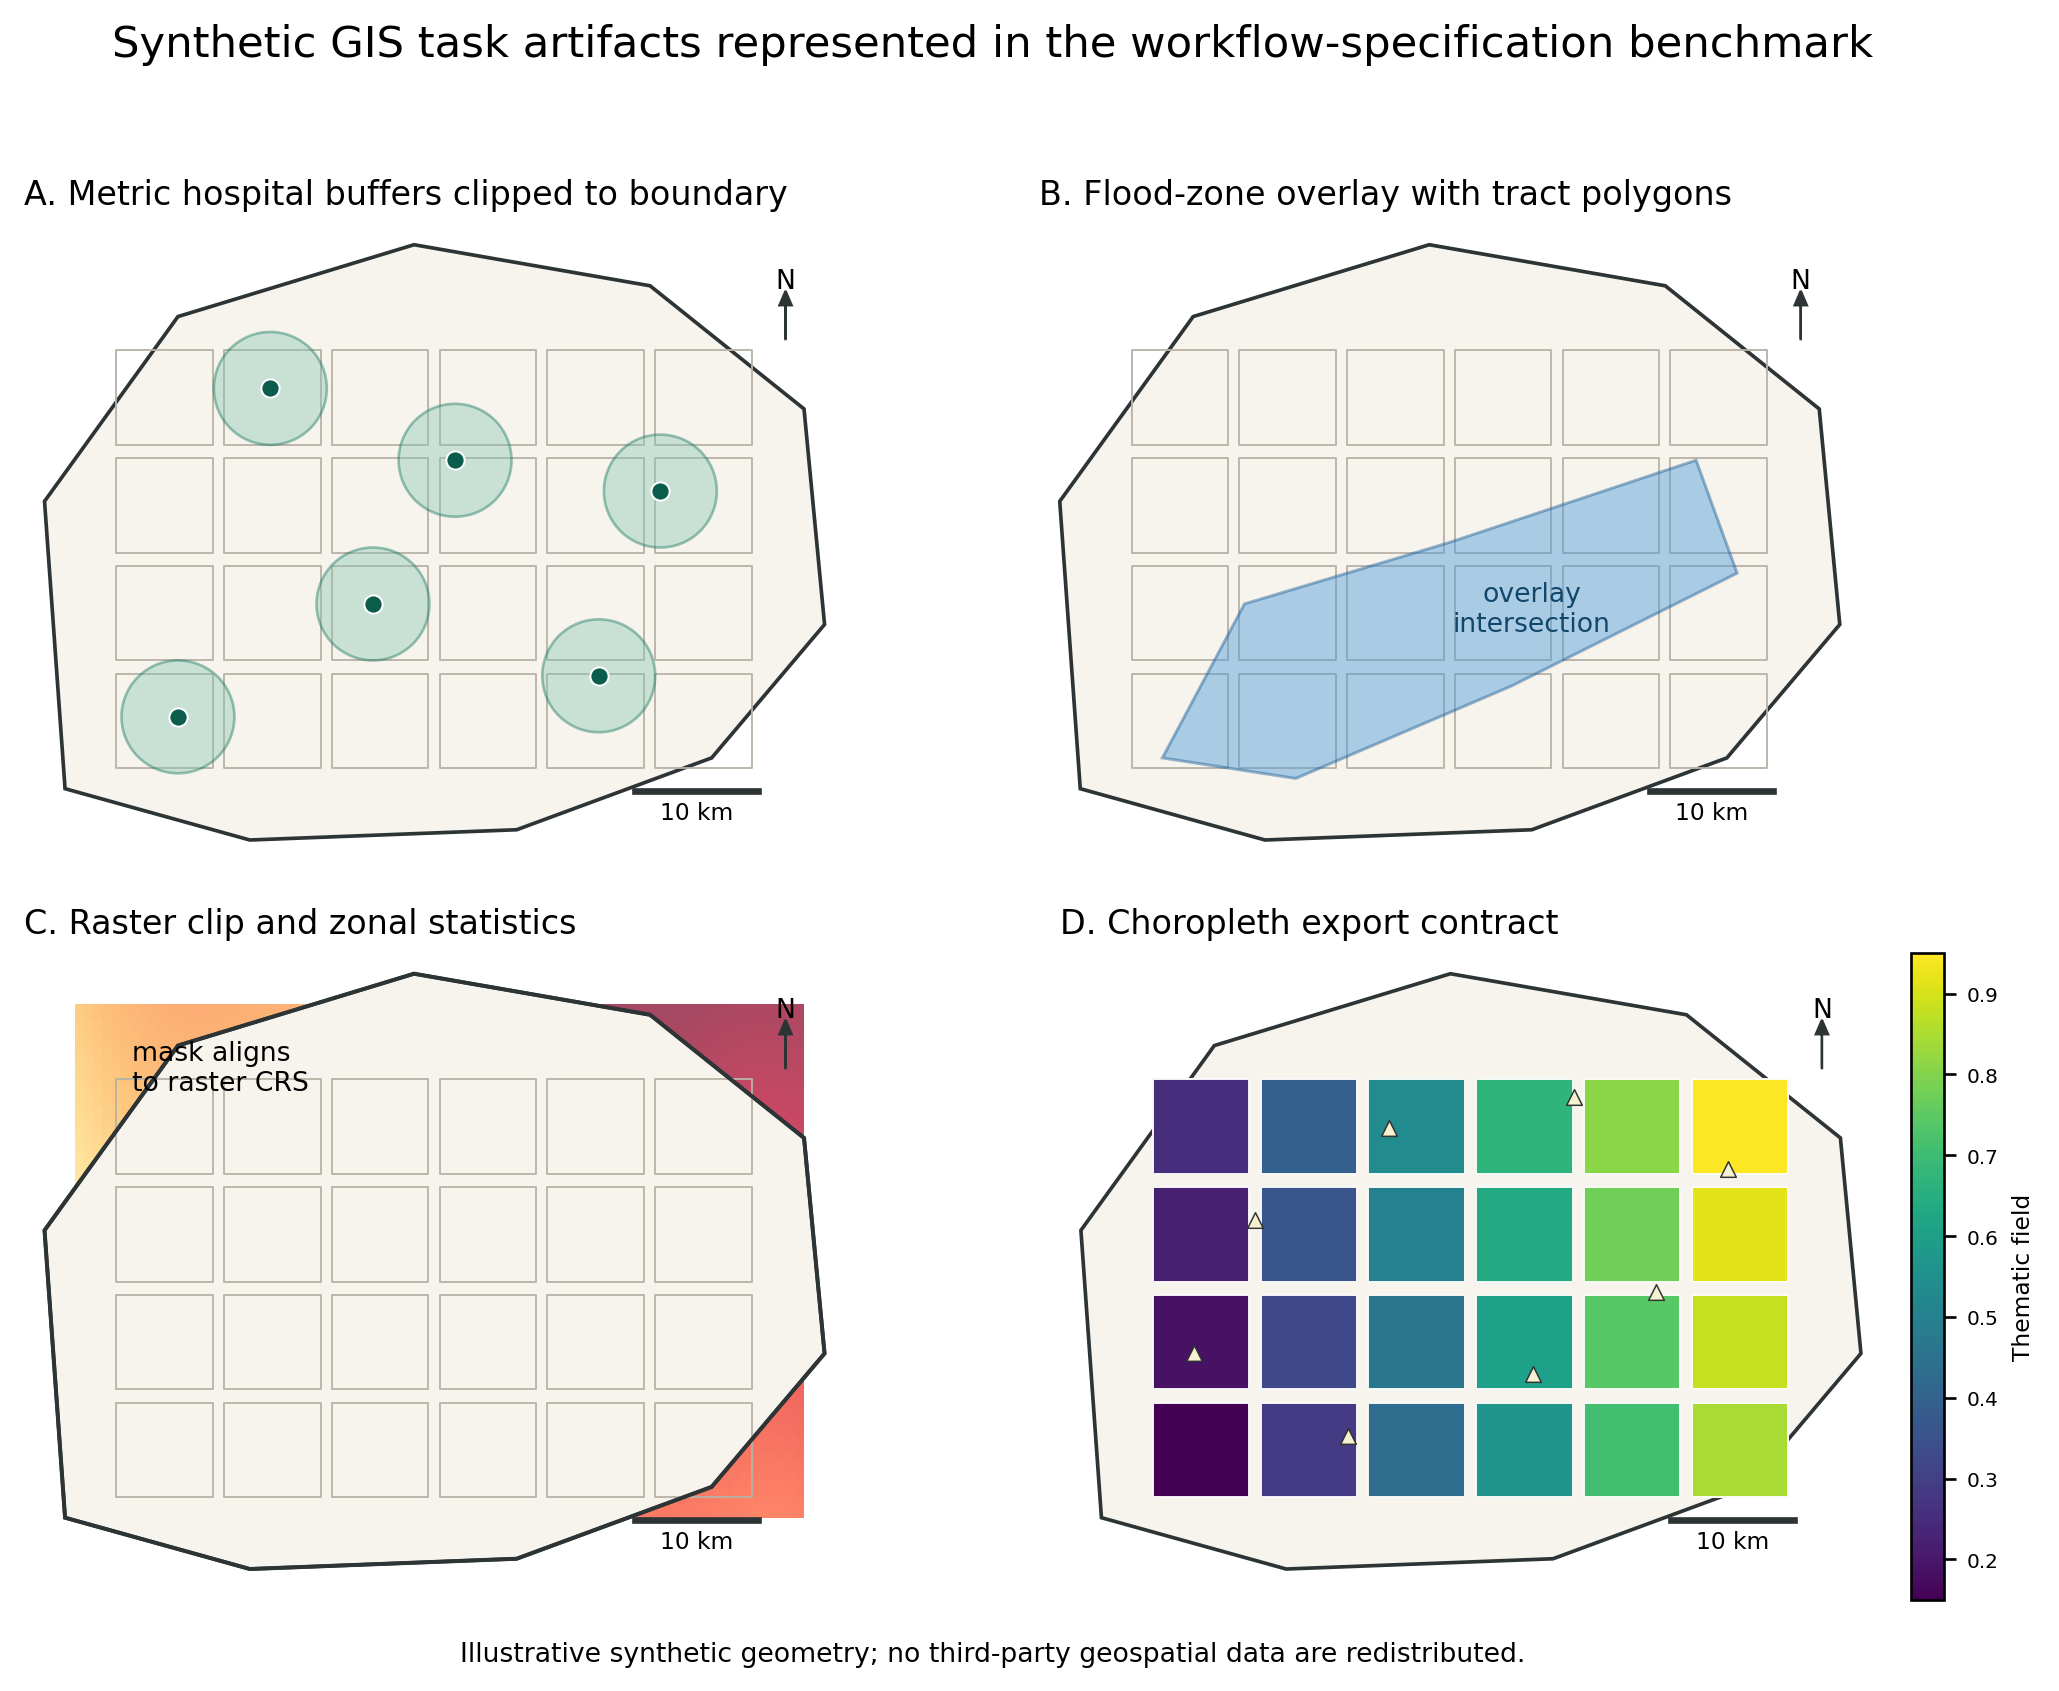
\includegraphics[width=0.98\textwidth]{figures/geo_task_suite_map_examples.png}
\caption{Synthetic GIS artifacts represented by the workflow-specification benchmark. The panels illustrate the geospatial operations that the JSON contracts must describe: metric hospital buffers clipped to a study boundary, flood-zone overlay with tract polygons, raster clipping and zonal statistics, and choropleth export with a thematic field and legend. The geometry is synthetic and is used only to visualize benchmark task semantics.}
\label{fig:geo-task-suite}
\end{figure}

Figure~\ref{fig:geo-operation-gallery} expands this view by showing one map-level example for each operation family. The gallery makes the diagnostic role of the task suite explicit: buffer tasks test distance and projection, overlay tasks test geometry interaction, point-count tasks test spatial aggregation, raster tasks test mask alignment, zonal tasks test raster-vector summaries, and choropleth tasks test cartographic output.

\begin{figure}[htbp]
\centering
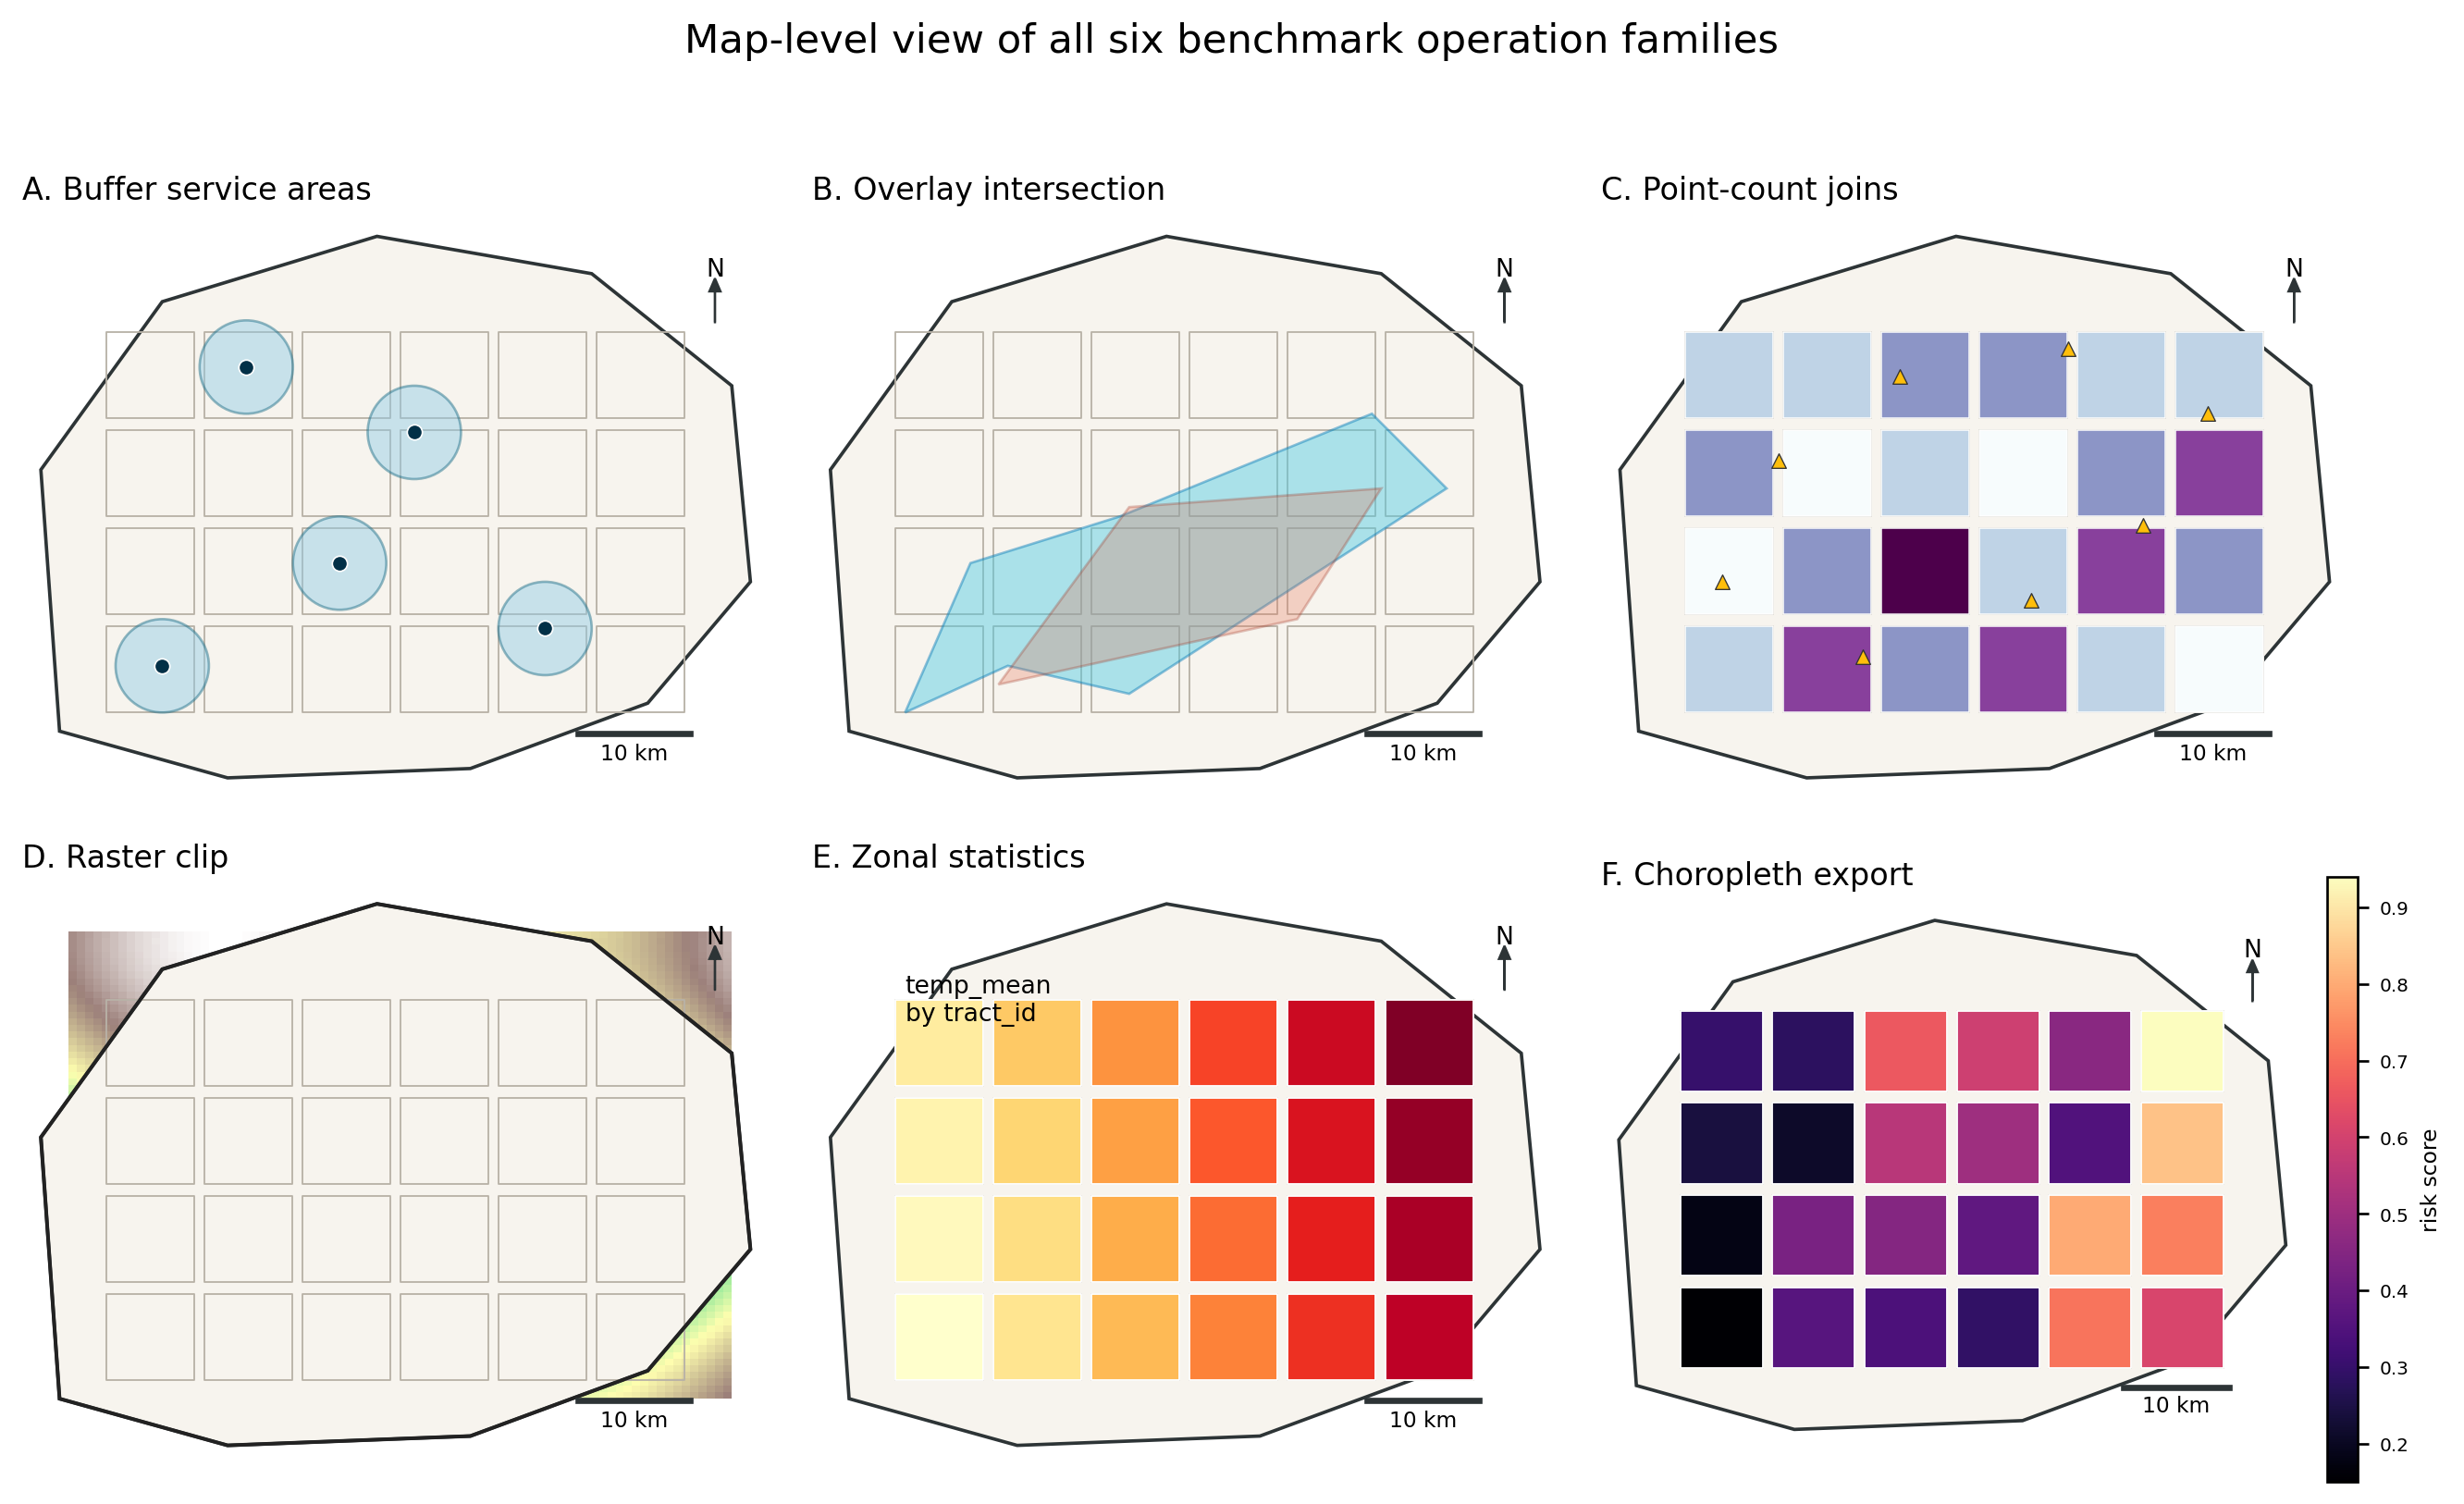
\includegraphics[width=0.98\textwidth]{figures/geo_operation_family_gallery.png}
\caption{Map-level gallery of the six benchmark operation families. The panels make explicit that the benchmark is not only a JSON-format task: it covers vector buffering, overlay, point-in-polygon aggregation, raster masking, zonal statistics, and choropleth map export.}
\label{fig:geo-operation-gallery}
\end{figure}

Figure~\ref{fig:geo-task-family} summarizes the same design at the family level. The six families are intentionally balanced as probes rather than treated as one homogeneous GIS task class.

\begin{figure}[htbp]
\centering
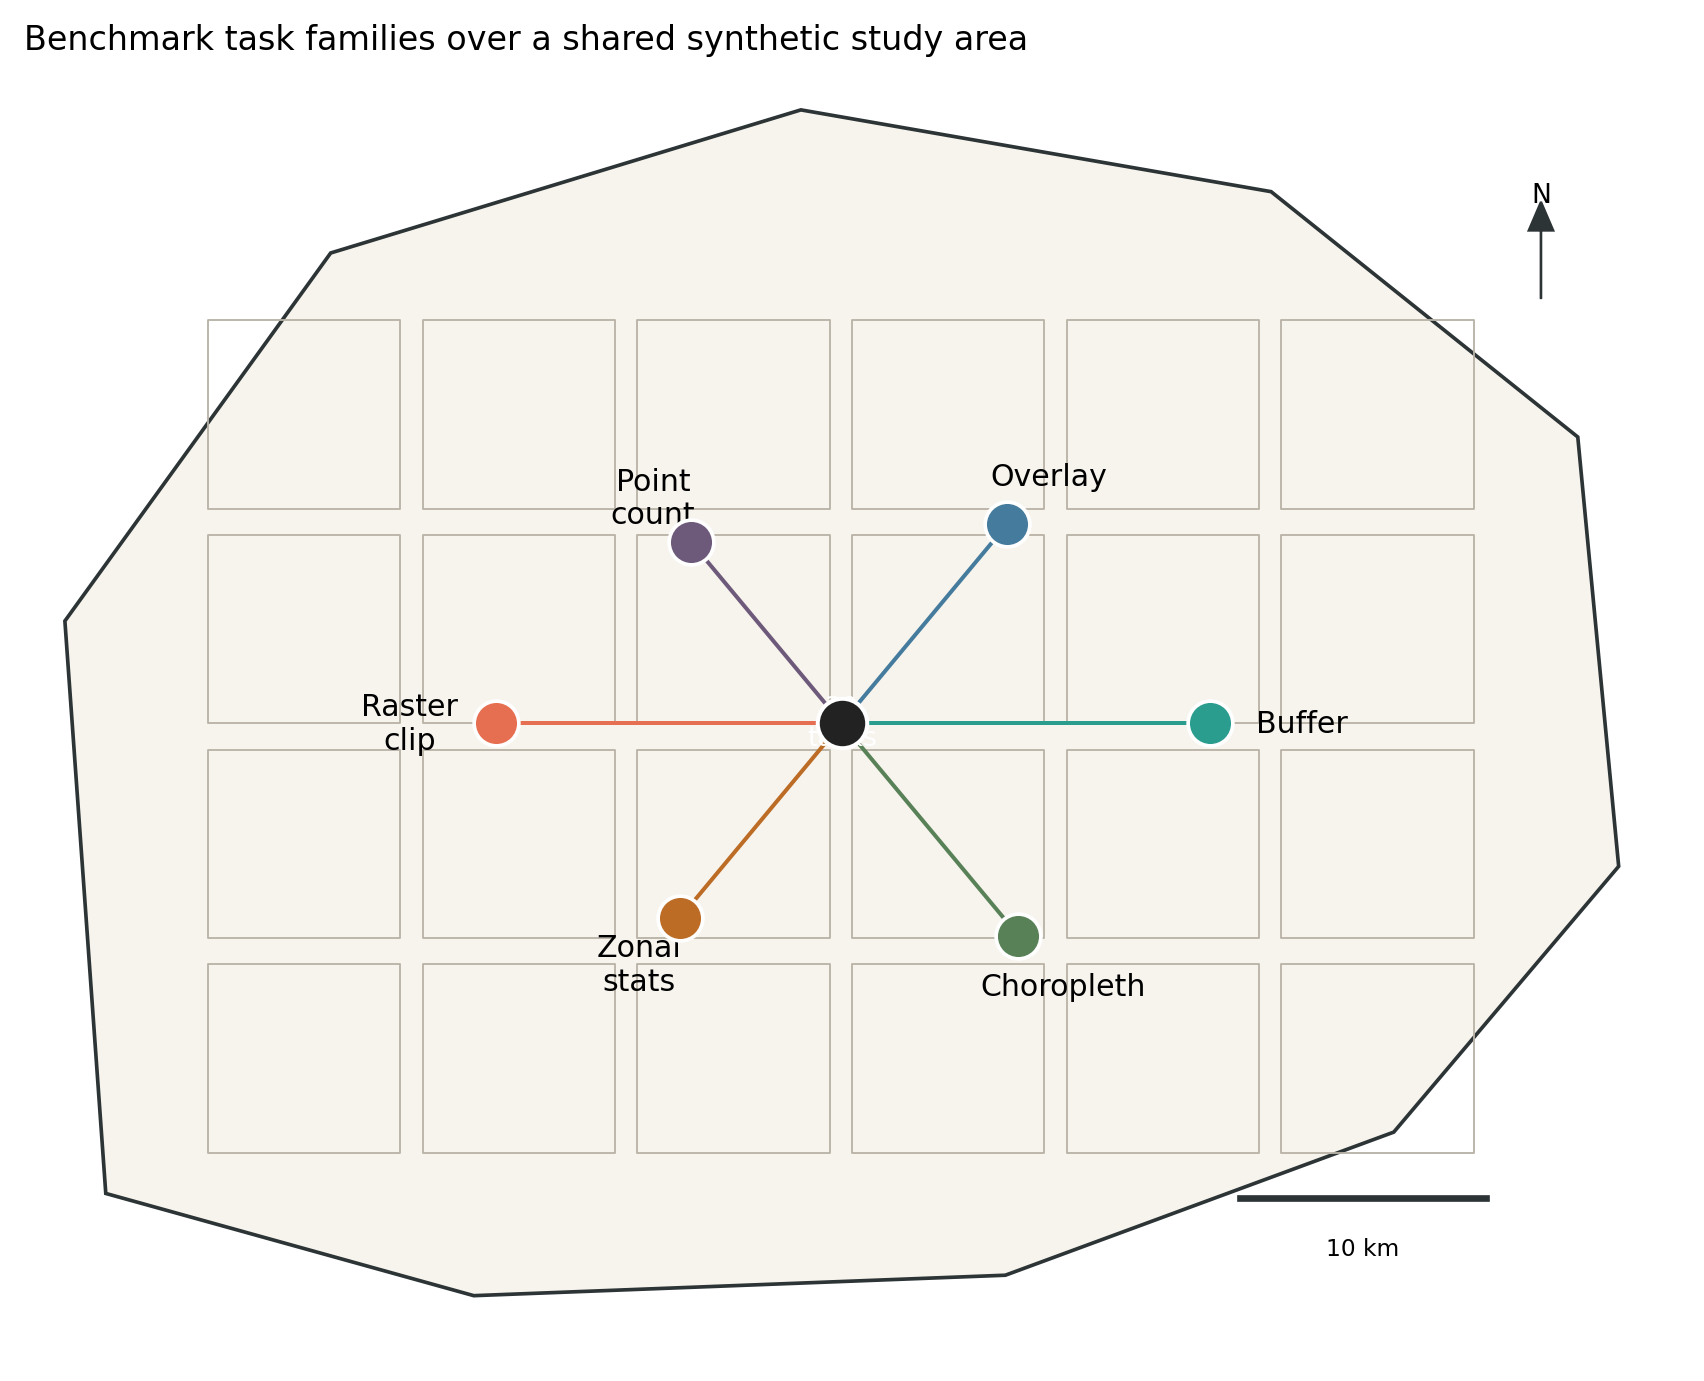
\includegraphics[width=0.78\textwidth]{figures/geo_task_family_coverage.png}
\caption{Geospatial coverage of the six task families in the 30-task suite. Each family probes a different part of the GIS workflow contract: measurement, overlay topology, point-in-polygon aggregation, raster-vector alignment, derived zonal fields, and cartographic export.}
\label{fig:geo-task-family}
\end{figure}

\subsection{Model panel, prompting modes, and workflow schema}

The first local model panel contains twelve Ollama models installed on the workstation:

\begin{quote}
qwen2.5-coder:1.5b, qwen2.5-coder:3b, qwen2.5-coder:7b, qwen2.5-coder:14b, qwen2.5-coder:32b, deepseek-coder:6.7b, qwen2.5:3b, qwen3:4b, llama3.2:3b, phi3:mini, mistral:7b, and gemma3:4b.
\end{quote}

The panel deliberately includes more than ten models and mixes coder-specialized models with compact general models. The goal is not only to rank models, but also to test which model families can satisfy a strict JSON workflow-contract protocol. Some models may be useful conversationally while failing the benchmark because they do not produce parseable structured specifications. In this design, that is a legitimate reliability outcome rather than an error to hide.

Each model is evaluated in three modes:

\begin{itemize}
\item \textit{Basic}: the model receives only the natural-language task, the task identifier, the expected operation type, the required output filename, the required fields, and the JSON schema.
\item \textit{Grounded}: the basic prompt is augmented with a data profile and a list of allowed GIS operations.
\item \textit{GeoGuard}: the grounded prompt is further augmented with validation rules for CRS handling, raster-vector alignment, schema preservation, geometry repair, and map quality.
\end{itemize}

The modes are designed to isolate the effect of grounding and validation. Basic mode tests whether a model can infer a plausible workflow from the user's request. Grounded mode tests whether explicit metadata reduces dataset and field hallucination. GeoGuard mode tests whether validation rules improve the model's planning for CRS, schema, and cartographic output requirements. Figure~\ref{fig:geo-validation-contract} visualizes the intended difference between these modes: the benchmark expects the model to move from a plausible but underspecified map operation toward a validated spatial workflow contract.

\begin{figure}[htbp]
\centering
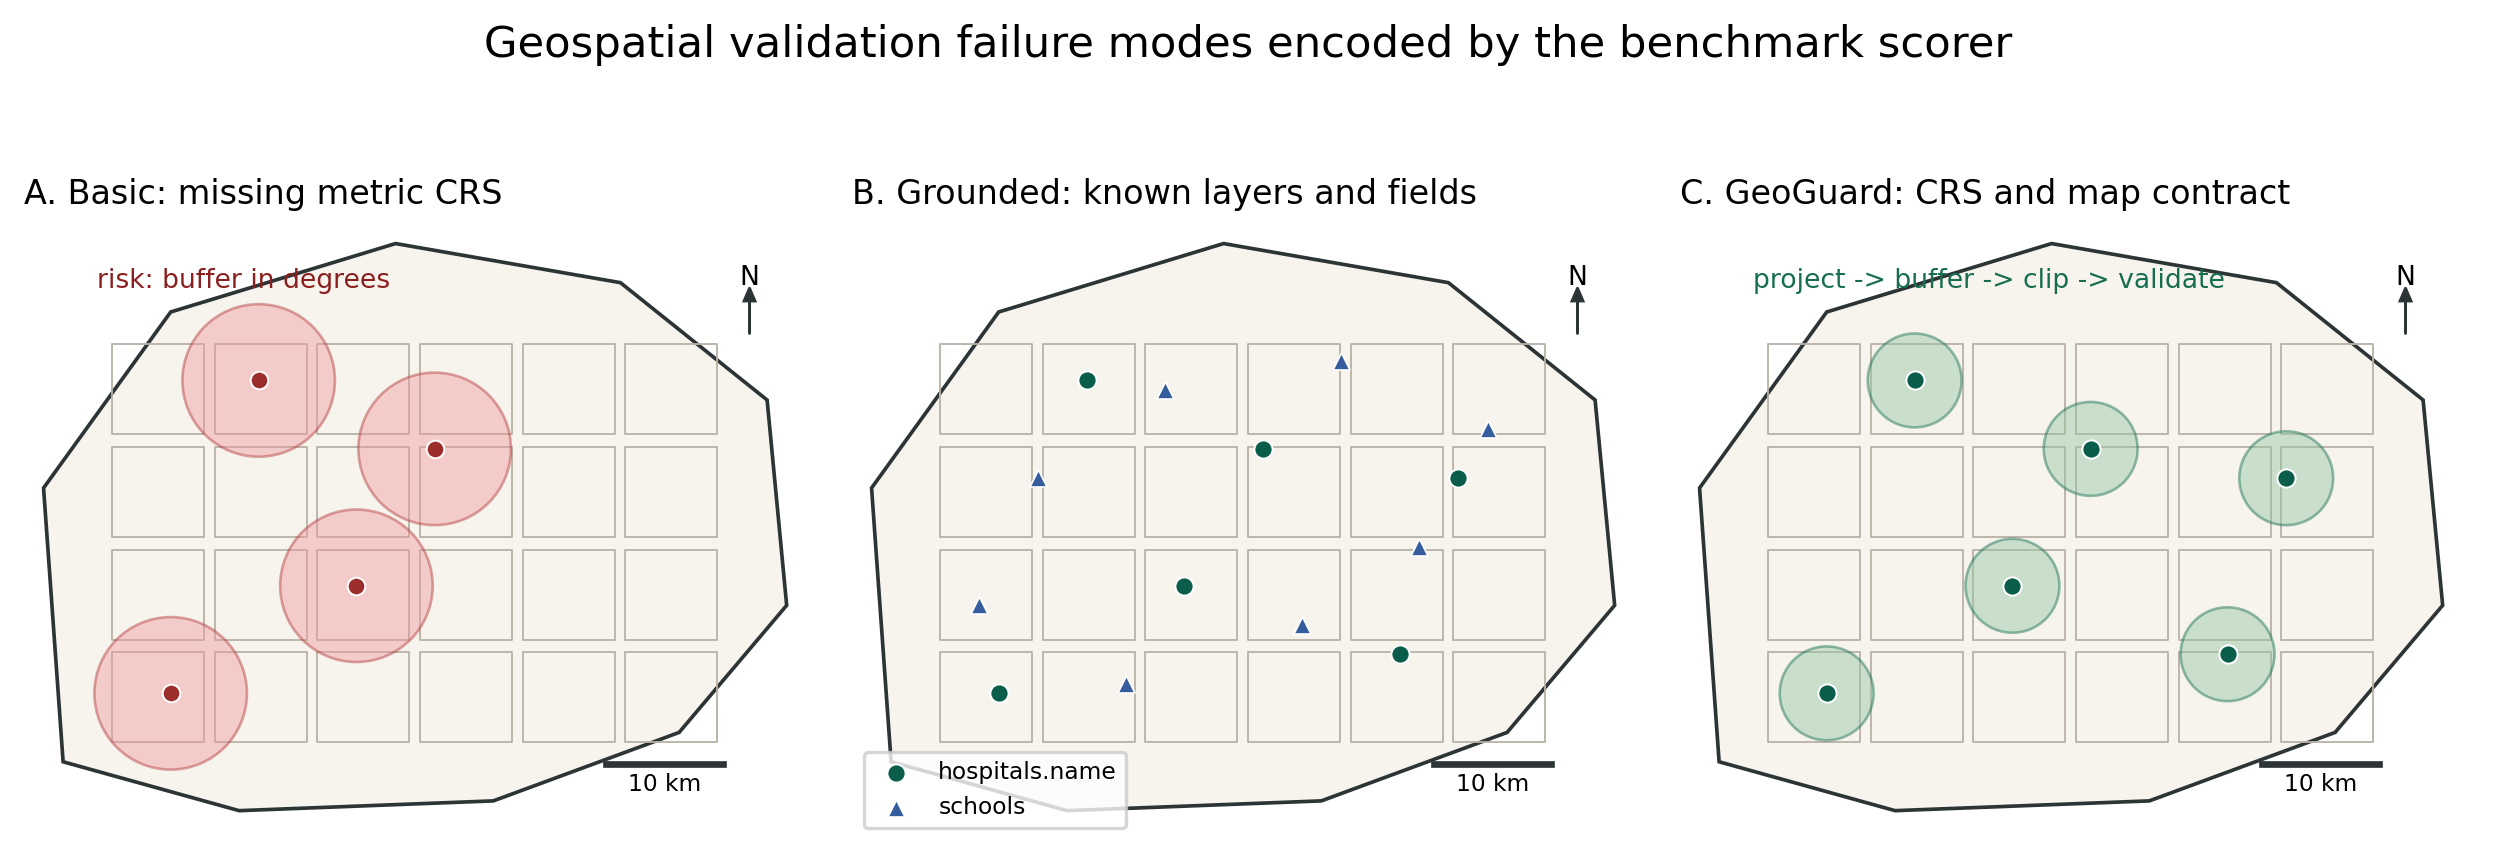
\includegraphics[width=0.98\textwidth]{figures/geo_validation_contract_examples.png}
\caption{Geospatial validation examples encoded by the benchmark scorer. Basic task-only prompting often leaves metric buffering, field provenance, and output map contracts implicit. Grounded prompting exposes known layers and fields, while GeoGuard adds checks for projection, clipping, schema preservation, and cartographic completeness before execution.}
\label{fig:geo-validation-contract}
\end{figure}

Every response is required to be a single JSON object with the following top-level keys: task identifier, operation, inputs, parameters, output, validation, and rationale. The output object must include a filename, output type, and required fields. The validation object may include CRS, schema, geometry, raster, and map-quality checks. The schema is intentionally simple enough for small local models, but strict enough to reveal malformed responses and implicit assumptions.

Figure~\ref{fig:geo-contract-anatomy} shows how this schema maps onto a GIS artifact. A correct contract links input layers, operation type, validation checks, output schema, and output artifact; omitting any one of these links can leave a downstream executor with an ambiguous or unsafe spatial plan.

\begin{figure}[htbp]
\centering
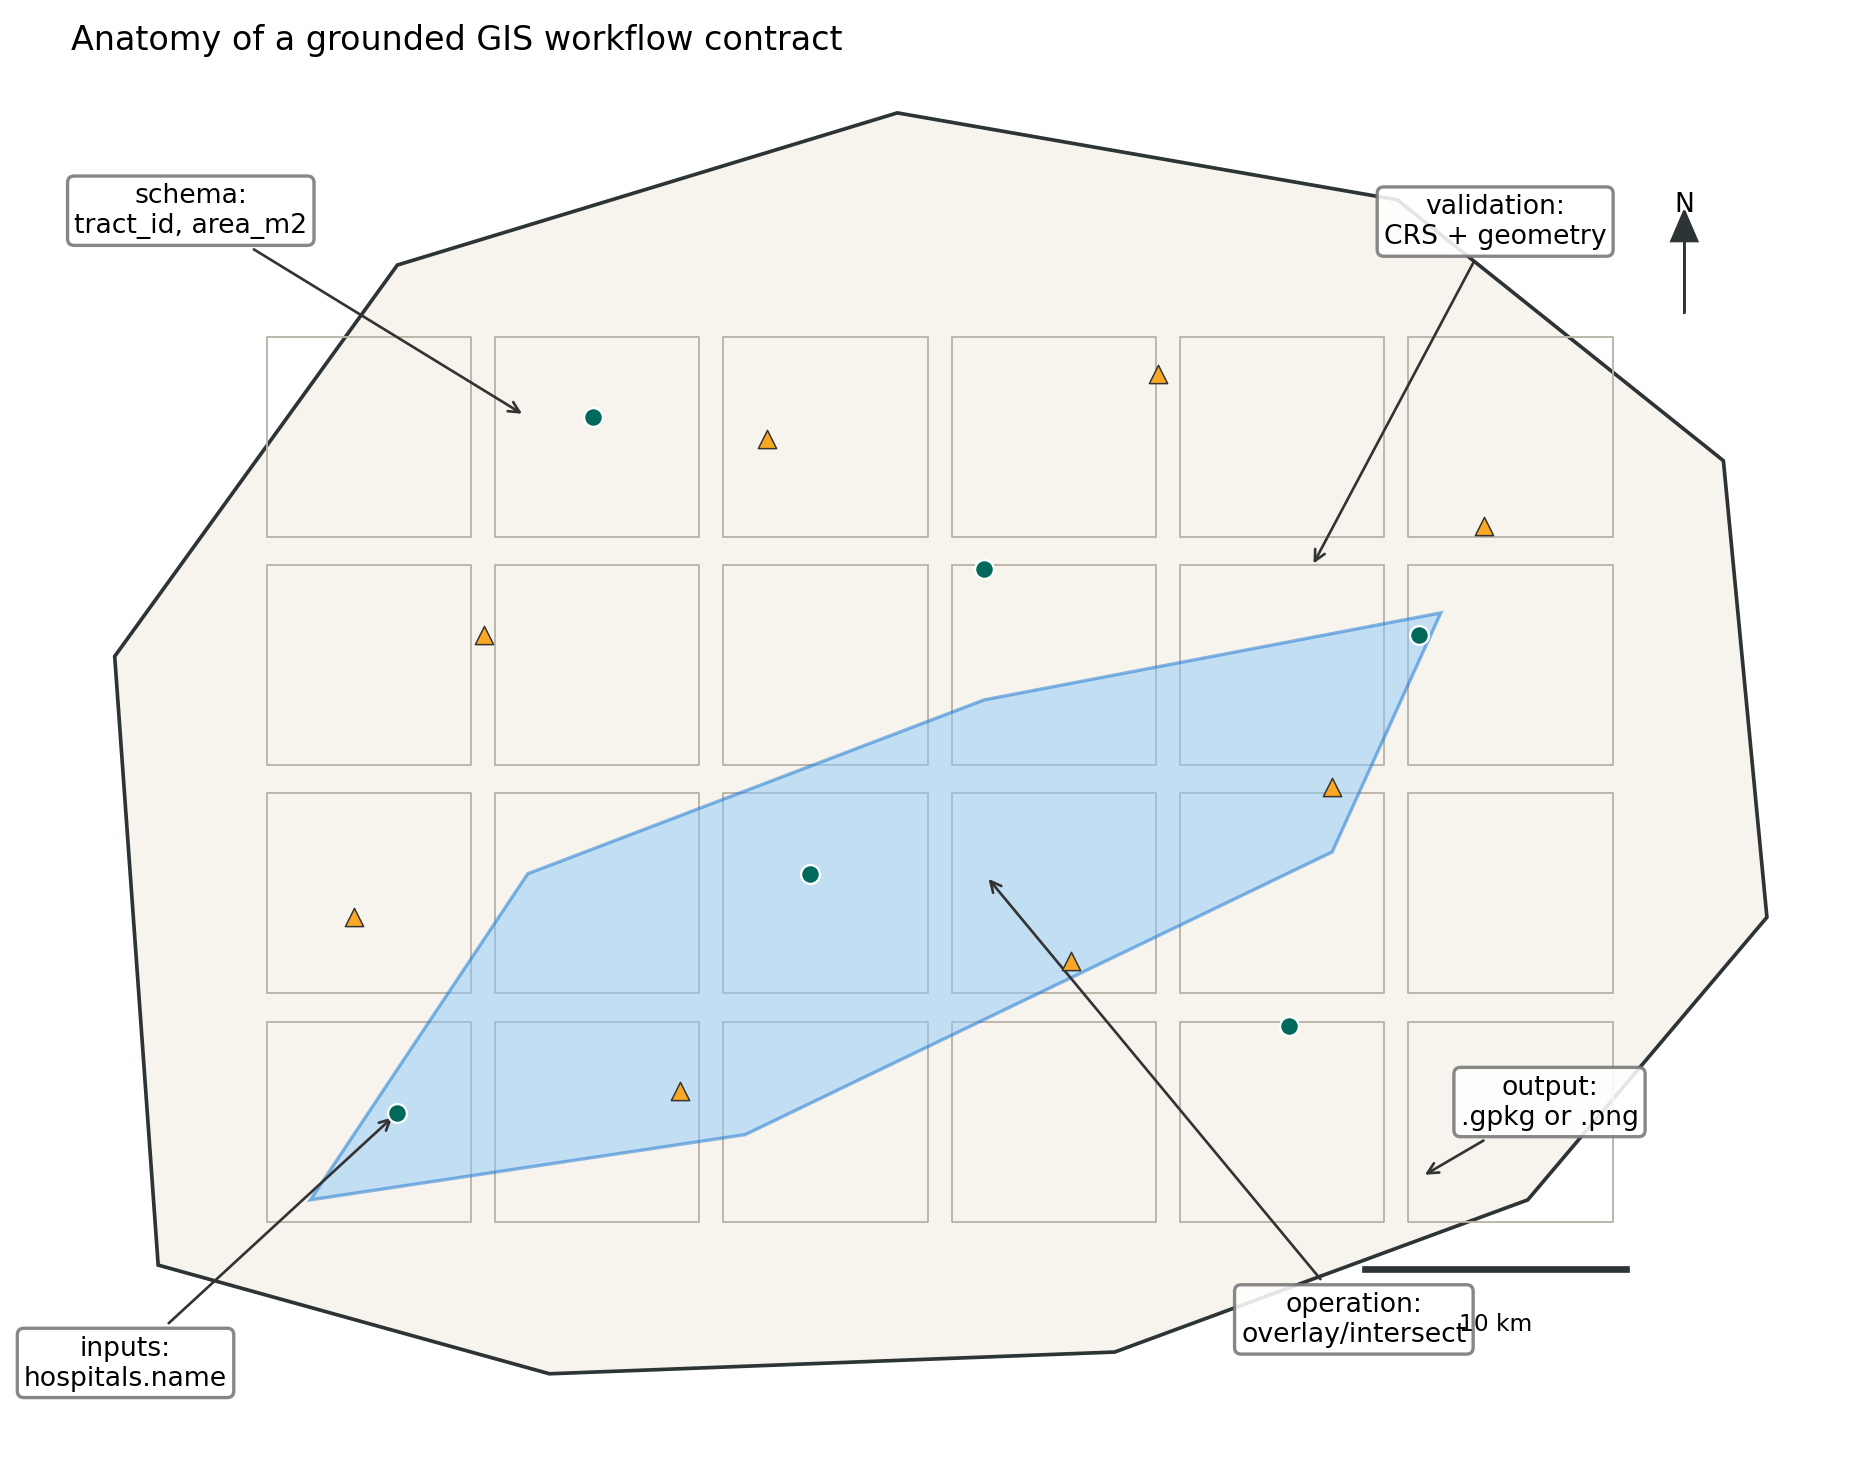
\includegraphics[width=0.82\textwidth]{figures/geo_workflow_contract_anatomy.png}
\caption{Anatomy of a grounded GIS workflow contract. A reliable specification must connect map layers, spatial operation, CRS and geometry validation, output schema, and artifact filename before a deterministic executor or renderer is allowed to run.}
\label{fig:geo-contract-anatomy}
\end{figure}

The scorer computes ten plan-level metrics:

\begin{itemize}
\item JSON validity: whether the response is parseable as a JSON object.
\item Tool validity: whether the operation matches the expected task type and belongs to the allowed operation set.
\item Data validity: whether all referenced layers are known layers.
\item Field validity: whether referenced or required fields exist or are created by the operation.
\item CRS plan: whether the plan includes an appropriate CRS strategy.
\item Schema plan: whether required output fields are declared.
\item Map plan: whether map-export tasks include title, legend, classification, color ramp, and source-note requirements.
\item Output name: whether the output filename matches the task.
\item Plan hallucination risk: an unweighted error fraction across tool, data, field, CRS, and filename checks.
\item Plan reliability score: a mean reliability summary across parseability, tool, data, field, CRS, schema, map, output, and inverse weighted hallucination risk.
\end{itemize}

The metrics are not intended as a final theory of GIS correctness. They are a reproducible first layer for comparing model behavior under explicit workflow contracts. Later phases can add execution-level and artifact-level metrics once valid specifications are passed to deterministic executors.

\section{Results}

\subsection{Experimental scope and aggregate mode effects}

The full experiment evaluates twelve local Ollama models over all 30 workflow tasks and three prompting modes. This yields 1080 attempted workflow specifications. Each model-mode pair contributes 30 task rows, and each mode contributes 360 task rows. The panel includes five qwen2.5-coder sizes, one DeepSeek coder model, and six compact or general local models. All models are evaluated under the same prompt protocol and JSON extraction rule; no model-specific prompt repair is applied.

All outputs are generated through the local Ollama HTTP API with deterministic temperature settings. Raw responses, parsed JSON specifications, generation manifests, task-level scores, and aggregate model summaries are written into the experiment track. The full summaries are mirrored into the manuscript table directory so that the manuscript can be rebuilt from recorded evidence rather than from manual notes.

Table~\ref{tab:mode-summary} and Figure~\ref{fig:mode-profile} summarize the full run by prompting mode. The dominant effect is the difference between task-only planning and metadata-grounded planning. In basic mode, mean data validity is only 0.053 because models frequently invent layer names, use generic filenames, or describe inputs informally. Grounded mode raises data validity to 0.761, increases JSON validity from 0.744 to 0.847, lowers weighted hallucination risk from 0.522 to 0.277, and raises plan reliability score from 0.547 to 0.751. The table gives the exact aggregate values, while the figure makes the mode-level profile easier to compare across metrics.

\begin{table}[htbp]
\centering
\caption{Aggregate full-run performance by prompting mode across twelve local Ollama models and 30 workflow tasks.}
\label{tab:mode-summary}
\small
\setlength{\tabcolsep}{5pt}
\begin{tabular}{lrrrrrrr}
\toprule
Mode & JSON valid & Data valid & Field valid & CRS plan & Map plan & WPHR & PRS \\
\midrule
Basic & 0.744 & 0.053 & 0.309 & 0.569 & 0.662 & 0.522 & 0.547 \\
Grounded & 0.847 & 0.761 & 0.562 & 0.674 & 0.824 & 0.277 & 0.751 \\
GeoGuard & 0.839 & 0.769 & 0.612 & 0.774 & 0.817 & 0.244 & 0.774 \\
\bottomrule
\end{tabular}
\end{table}

Table~\ref{tab:mode-summary} shows that grounding is the main discontinuity in the experiment. The basic-to-grounded jump in data validity is far larger than the grounded-to-GeoGuard change, which indicates that most dataset hallucination is caused by missing data context rather than by weak reasoning alone. GeoGuard's value is narrower but still important: it improves CRS planning and field validity while slightly lowering map-plan score, suggesting that validation-heavy prompts help spatial correctness more than cartographic design completeness. This pattern supports a two-layer prompt design: provide metadata first, then add validation rules for operations where CRS, schema, or raster-vector alignment can change the geographic meaning of the result.

\begin{figure}[htbp]
\centering
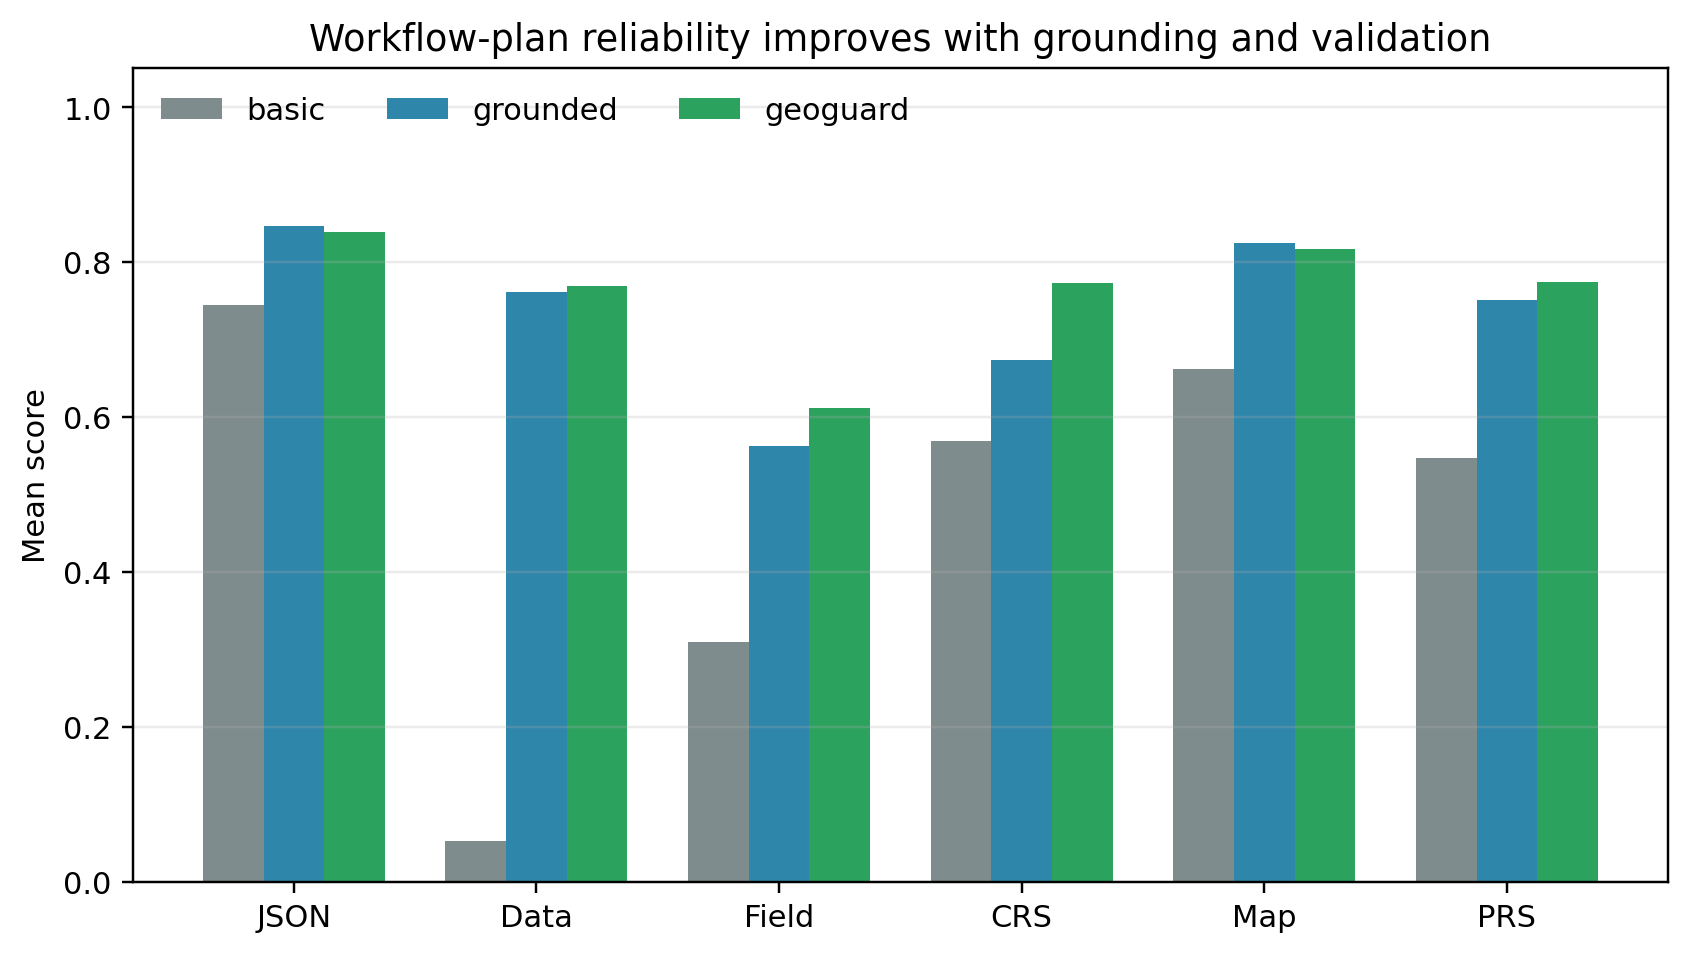
\includegraphics[width=0.92\textwidth]{figures/full_mode_metric_profile.png}
\caption{Mean metric profile by prompting mode across 1080 attempted specifications. Metadata grounding primarily improves data and field validity, while GeoGuard-style validation produces the strongest CRS-planning gains.}
\label{fig:mode-profile}
\end{figure}

The GeoGuard condition produces the strongest CRS-planning effect. Grounded mode tells models what data and tools exist, but it does not always force them to reason consistently about metric buffers, raster masks, or projected area calculations. Adding validation rules raises mean CRS planning from 0.674 in grounded mode to 0.774 in GeoGuard mode and reduces weighted hallucination risk from 0.277 to 0.244. The overall plan reliability increase from grounded to GeoGuard is smaller than the basic-to-grounded jump because some compact models remain unable to satisfy the strict JSON protocol and because map-export tasks expose field and cartographic-plan weaknesses that validation rules do not fully resolve.

\subsection{Execution readiness, repair, and stress tests}

To make the benchmark more than a descriptive leaderboard, a second analysis treats each model-task pair as a paired unit and estimates mode effects with bootstrap confidence intervals. Table~\ref{tab:bootstrap-mode-effects} shows that the grounded-minus-basic effect is large for data validity, field validity, map planning, WPHR, PRS, and execution readiness. The GeoGuard-minus-grounded effect is narrower but still positive for CRS planning, field validity, WPHR, PRS, and execution readiness. This distinction matters substantively: grounding is the main anti-hallucination intervention, while GeoGuard is a spatial-validity intervention.

\begin{table}[htbp]
\centering
\caption{Paired mode effects with bootstrap 95\% confidence intervals across 360 model-task units.}
\label{tab:bootstrap-mode-effects}
\scriptsize
\setlength{\tabcolsep}{3pt}
\begin{tabular}{lrrr}
\toprule
Metric & Grounded--Basic & GeoGuard--Grounded & GeoGuard--Basic \\
\midrule
Data validity & 0.7083 [0.6611, 0.7556] & 0.0083 [-0.0194, 0.0361] & 0.7167 [0.6722, 0.7639] \\
Field validity & 0.2535 [0.2020, 0.3083] & 0.0494 [0.0225, 0.0778] & 0.3029 [0.2499, 0.3567] \\
CRS plan & 0.1042 [0.0653, 0.1458] & 0.1000 [0.0653, 0.1375] & 0.2042 [0.1597, 0.2514] \\
Schema plan & 0.0986 [0.0569, 0.1417] & 0.0269 [-0.0019, 0.0574] & 0.1255 [0.0833, 0.1685] \\
Map plan & 0.1622 [0.1228, 0.2022] & -0.0078 [-0.0317, 0.0172] & 0.1544 [0.1128, 0.1972] \\
WPHR & -0.2454 [-0.2750, -0.2158] & -0.0327 [-0.0541, -0.0118] & -0.2781 [-0.3119, -0.2442] \\
PRS & 0.2040 [0.1751, 0.2335] & 0.0230 [0.0024, 0.0442] & 0.2270 [0.1937, 0.2602] \\
Execution-ready & 0.2528 [0.2083, 0.2972] & 0.0944 [0.0611, 0.1306] & 0.3472 [0.2972, 0.3972] \\
\bottomrule
\end{tabular}
\end{table}


The execution-readiness gate is intentionally stricter than the scalar PRS score. A contract is counted as execution-ready only when it is parseable, names the correct operation, references known data, uses a complete output filename, contains an acceptable CRS plan, declares enough schema and field information, and satisfies the map-plan threshold when a PNG export is requested. Table~\ref{tab:execution-readiness} shows that only 6 of 360 basic-mode rows pass this gate. Grounded prompting raises the count to 97, and GeoGuard raises it to 131. The dominant blocker also changes: in basic mode the first blocker is almost always data hallucination, while in grounded and GeoGuard modes the remaining bottleneck is field/schema planning.

\begin{table}[htbp]
\centering
\caption{Execution-readiness gate by prompting mode. Counts are out of 360 rows per mode.}
\label{tab:execution-readiness}
\small
\begin{tabular}{lrrrrl}
\toprule
Mode & Ready & Rate & Strict & Strict rate & Top blocker \\
\midrule
Basic & 6 & 0.017 & 6 & 0.017 & data (248) \\
Grounded & 97 & 0.269 & 92 & 0.256 & field (128) \\
GeoGuard & 131 & 0.364 & 124 & 0.344 & field (116) \\
\bottomrule
\end{tabular}
\end{table}


Table~\ref{tab:family-execution-readiness} gives the same gate by task family. Raster clipping and buffer workflows show the largest readiness gains because their central risks, raster-mask alignment and metric buffering, are directly expressible as validation rules. Overlay workflows remain difficult because they require both correct layer pairing and output-field handling; choropleth workflows improve but remain limited by thematic-field and map-contract decisions. The readiness gate therefore connects plan-level scoring to an operational question: which model outputs are sufficiently specified to hand to a deterministic GIS executor without human repair?

\begin{table}[htbp]
\centering
\caption{Execution-readiness rate by task family and prompting mode. Counts are out of 60 rows per family-mode pair.}
\label{tab:family-execution-readiness}
\small
\begin{tabular}{lrrrrrr}
\toprule
Family & Basic & Grounded & GeoGuard & Basic n & Grounded n & GeoGuard n \\
\midrule
Buffer & 0.000 & 0.183 & 0.617 & 0 & 11 & 37 \\
Choropleth & 0.000 & 0.283 & 0.350 & 0 & 17 & 21 \\
Overlay & 0.000 & 0.000 & 0.033 & 0 & 0 & 2 \\
Point-count & 0.000 & 0.317 & 0.317 & 0 & 19 & 19 \\
Raster & 0.100 & 0.667 & 0.700 & 6 & 40 & 42 \\
Zonal & 0.000 & 0.167 & 0.167 & 0 & 10 & 10 \\
\bottomrule
\end{tabular}
\end{table}


The execution-readiness gate is conservative, but it can make the empirical basis look smaller than the generated panel. To test whether the planning metrics remain informative beyond the gate, a second execution analysis runs the deterministic executor over the full 1080-contract cohort. Contracts that fail to parse or cannot be bound to required layer roles are counted as non-executable rather than removed. This full-cohort analysis produces 43 valid artifacts from basic prompting, 230 from grounded prompting, and 233 from GeoGuard prompting (Table~\ref{tab:full-cohort-execution}). The result preserves the same qualitative finding as the planning scores: task-only prompts rarely contain enough grounded information for execution, while metadata and validation prompts turn many more specifications into runnable GIS artifacts.

\begin{table}[htbp]
\centering
\caption{Full-cohort deterministic execution across all 1080 attempted workflow contracts. Valid-per-attempt treats malformed, unbound, and execution-failed contracts as failures.}
\label{tab:full-cohort-execution}
\small
\setlength{\tabcolsep}{4pt}
\begin{tabular}{lrrrrrr}
\toprule
Mode & Attempted & JSON valid & Ready & Compatible & Valid artifacts & Valid/attempt \\
\midrule
Basic & 360 & 268 & 6 & 43 & 43 & 0.119 \\
Grounded & 360 & 305 & 97 & 231 & 230 & 0.639 \\
GeoGuard & 360 & 302 & 131 & 235 & 233 & 0.647 \\
\bottomrule
\end{tabular}
\end{table}

Figure~\ref{fig:execution-outcomes-mode} visualizes the same full-cohort result as outcome counts, making the denominator transparent across valid artifacts, malformed contracts, and role-binding failures.

\begin{figure}[htbp]
\centering
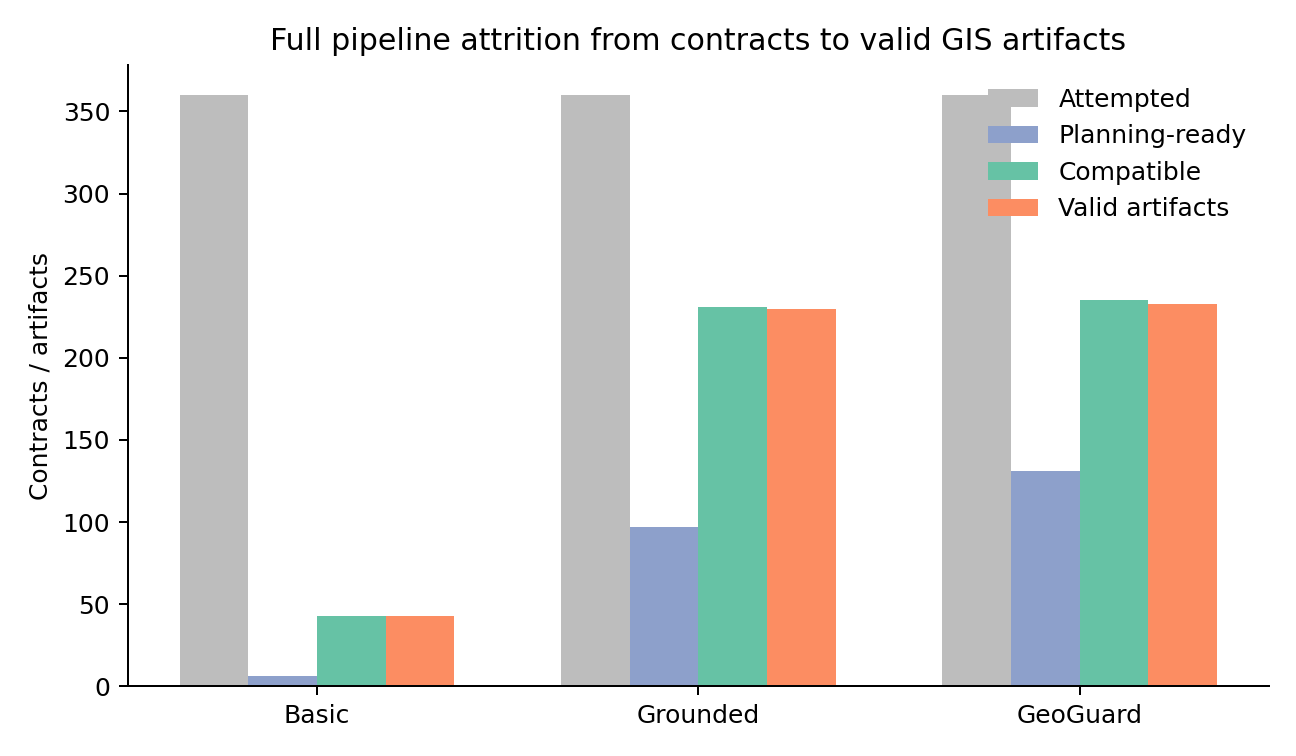
\includegraphics[width=0.86\textwidth]{figures/execution_outcomes_by_mode.png}
\caption{Full-cohort execution outcomes by prompting mode. The denominator includes all generated contracts, including malformed JSON and contracts that cannot bind required layer roles.}
\label{fig:execution-outcomes-mode}
\end{figure}

Because each mode is evaluated on the same model--task pairs, the execution outcomes can also be compared as paired differences. Bootstrap intervals over the 360 paired units show a large execution gain for both grounded prompting and GeoGuard over basic prompting, while the GeoGuard-minus-grounded difference is small and overlaps zero (Table~\ref{tab:paired-execution-comparisons}). This paired analysis avoids treating the three modes as independent samples; the units are the same tasks and models under different prompting conditions.

\begin{table}[htbp]
\centering
\caption{Paired bootstrap comparisons for strict full-cohort valid-artifact outcomes. Mean differences are valid-artifact probability differences over the same 360 model--task units per comparison.}
\label{tab:paired-execution-comparisons}
\small
\setlength{\tabcolsep}{3pt}
\begin{tabular}{lrrrrr}
\toprule
Comparison & Mean diff. & 95\% CI & Positive & Negative & Ties \\
\midrule
Grounded minus Basic & 0.519 & [0.469, 0.569] & 187 & 0 & 173 \\
GeoGuard minus Basic & 0.528 & [0.475, 0.578] & 190 & 0 & 170 \\
GeoGuard minus Grounded & 0.008 & [-0.019, 0.036] & 14 & 11 & 335 \\
Repair minus strict, Basic & 0.625 & [0.572, 0.675] & 225 & 0 & 135 \\
Repair minus strict, Grounded & 0.206 & [0.164, 0.247] & 74 & 0 & 286 \\
Repair minus strict, GeoGuard & 0.189 & [0.150, 0.231] & 68 & 0 & 292 \\
\bottomrule
\end{tabular}
\end{table}

A bounded repair analysis tests whether failures are mainly shallow role-binding omissions rather than wrong spatial algorithms. A deterministic repair policy supplies missing layer-role defaults only when the operation family and task contract determine the required role unambiguously; it does not change the declared operation, output filename, or generated fields. Under this bounded policy, valid artifacts increase from 43 to 268 in basic mode, from 230 to 304 in grounded mode, and from 233 to 301 in GeoGuard mode (Table~\ref{tab:repair-execution}). This analysis is diagnostic rather than a replacement for the stricter gate: it shows that many full-cohort failures are caused by incomplete interface binding rather than by an impossible GIS operation.

\begin{table}[htbp]
\centering
\caption{Bounded role-default repair for the full execution cohort. Repair is deterministic and limited to unambiguous layer-role binding.}
\label{tab:repair-execution}
\small
\setlength{\tabcolsep}{4pt}
\begin{tabular}{lrrrrr}
\toprule
Mode & Attempted & Strict valid & Repaired valid & Rescued & Repaired rate \\
\midrule
Basic & 360 & 43 & 268 & 225 & 0.744 \\
Grounded & 360 & 230 & 304 & 74 & 0.844 \\
GeoGuard & 360 & 233 & 301 & 68 & 0.836 \\
\bottomrule
\end{tabular}
\end{table}

The repair effect is not uniform across task families. Choropleth export and zonal statistics gain the most rescued artifacts, while overlay intersection gains less because a larger share of overlay contracts are already strict-valid (Table~\ref{tab:repair-family}). This pattern supports a narrower interpretation of the repair experiment: it diagnoses interface-binding weakness, especially in map-export and aggregation tasks, rather than showing that all failed plans can be corrected automatically.

\begin{table}[htbp]
\centering
\caption{Bounded repair by task family across the full execution cohort. Rescued artifacts are contracts that were not strict-valid but became valid after deterministic role-default binding.}
\label{tab:repair-family}
\small
\setlength{\tabcolsep}{3pt}
\begin{tabular}{lrrrrr}
\toprule
Task family & Attempted & Strict valid & Repaired valid & Rescued & Repaired rate \\
\midrule
Buffer service area & 180 & 87 & 133 & 46 & 0.739 \\
Choropleth export & 180 & 54 & 142 & 88 & 0.789 \\
Overlay intersection & 180 & 118 & 151 & 33 & 0.839 \\
Point-count join & 180 & 88 & 156 & 68 & 0.867 \\
Raster clip & 180 & 91 & 145 & 54 & 0.806 \\
Zonal statistics & 180 & 68 & 146 & 78 & 0.811 \\
\bottomrule
\end{tabular}
\end{table}

Figure~\ref{fig:role-default-repair-examples} shows representative repaired artifacts and clarifies the diagnostic nature of this repair step: it fills deterministic role bindings but does not ask the model to regenerate the workflow.

\begin{figure}[htbp]
\centering
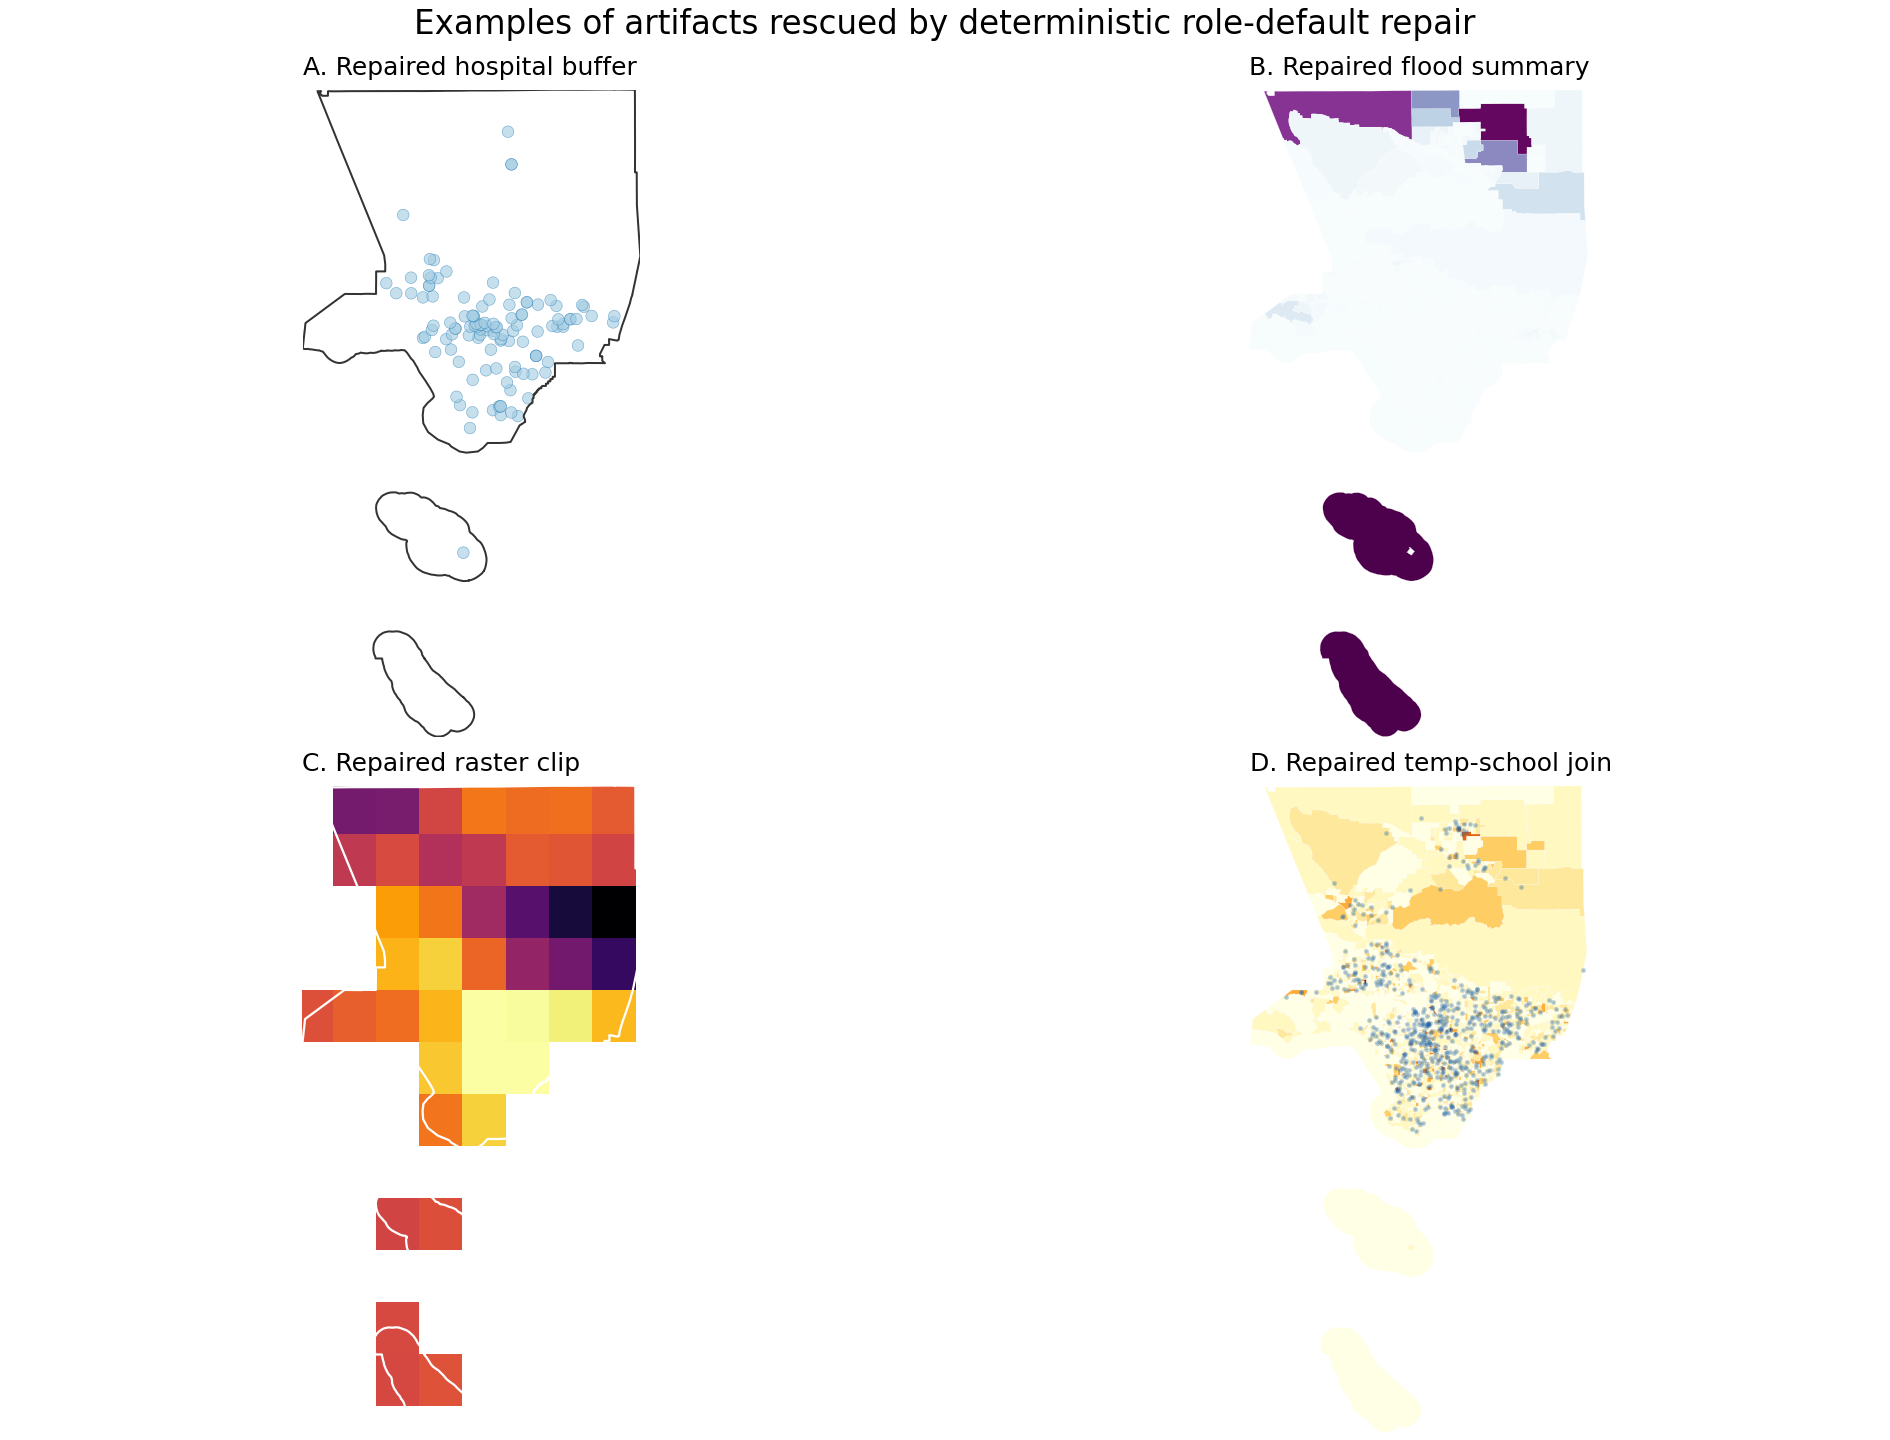
\includegraphics[width=0.92\textwidth]{figures/role_default_repair_map_examples.png}
\caption{Representative artifacts produced after bounded role-default repair. The repair policy fills only deterministic layer-role bindings, making the examples a diagnostic for contract-interface omissions rather than a second LLM generation pass.}
\label{fig:role-default-repair-examples}
\end{figure}

To avoid evaluating only against one dataset binding, the repaired execution cohort is also run against a synthetic data profile with different geometry scale, feature counts, raster transform, and artifact sizes. The valid-artifact counts are identical by mode because the same contracts satisfy the same operation-level requirements, but artifact-size signatures differ substantially across profiles. For example, the median valid buffer output changes from 116 rows in the GeoGuard Los Angeles County profile to 6 rows in the synthetic profile, and the median valid choropleth artifact changes from 130{,}511 pixels to 38{,}558 pixels. This confirms that the second run regenerates outputs over a different geospatial profile rather than reusing the first execution artifacts. Figure~\ref{fig:map-case-studies-geoguard} gives representative valid artifacts from the GeoGuard condition, connecting the contract scores to concrete vector, raster, and map outputs.

\begin{figure}[htbp]
\centering
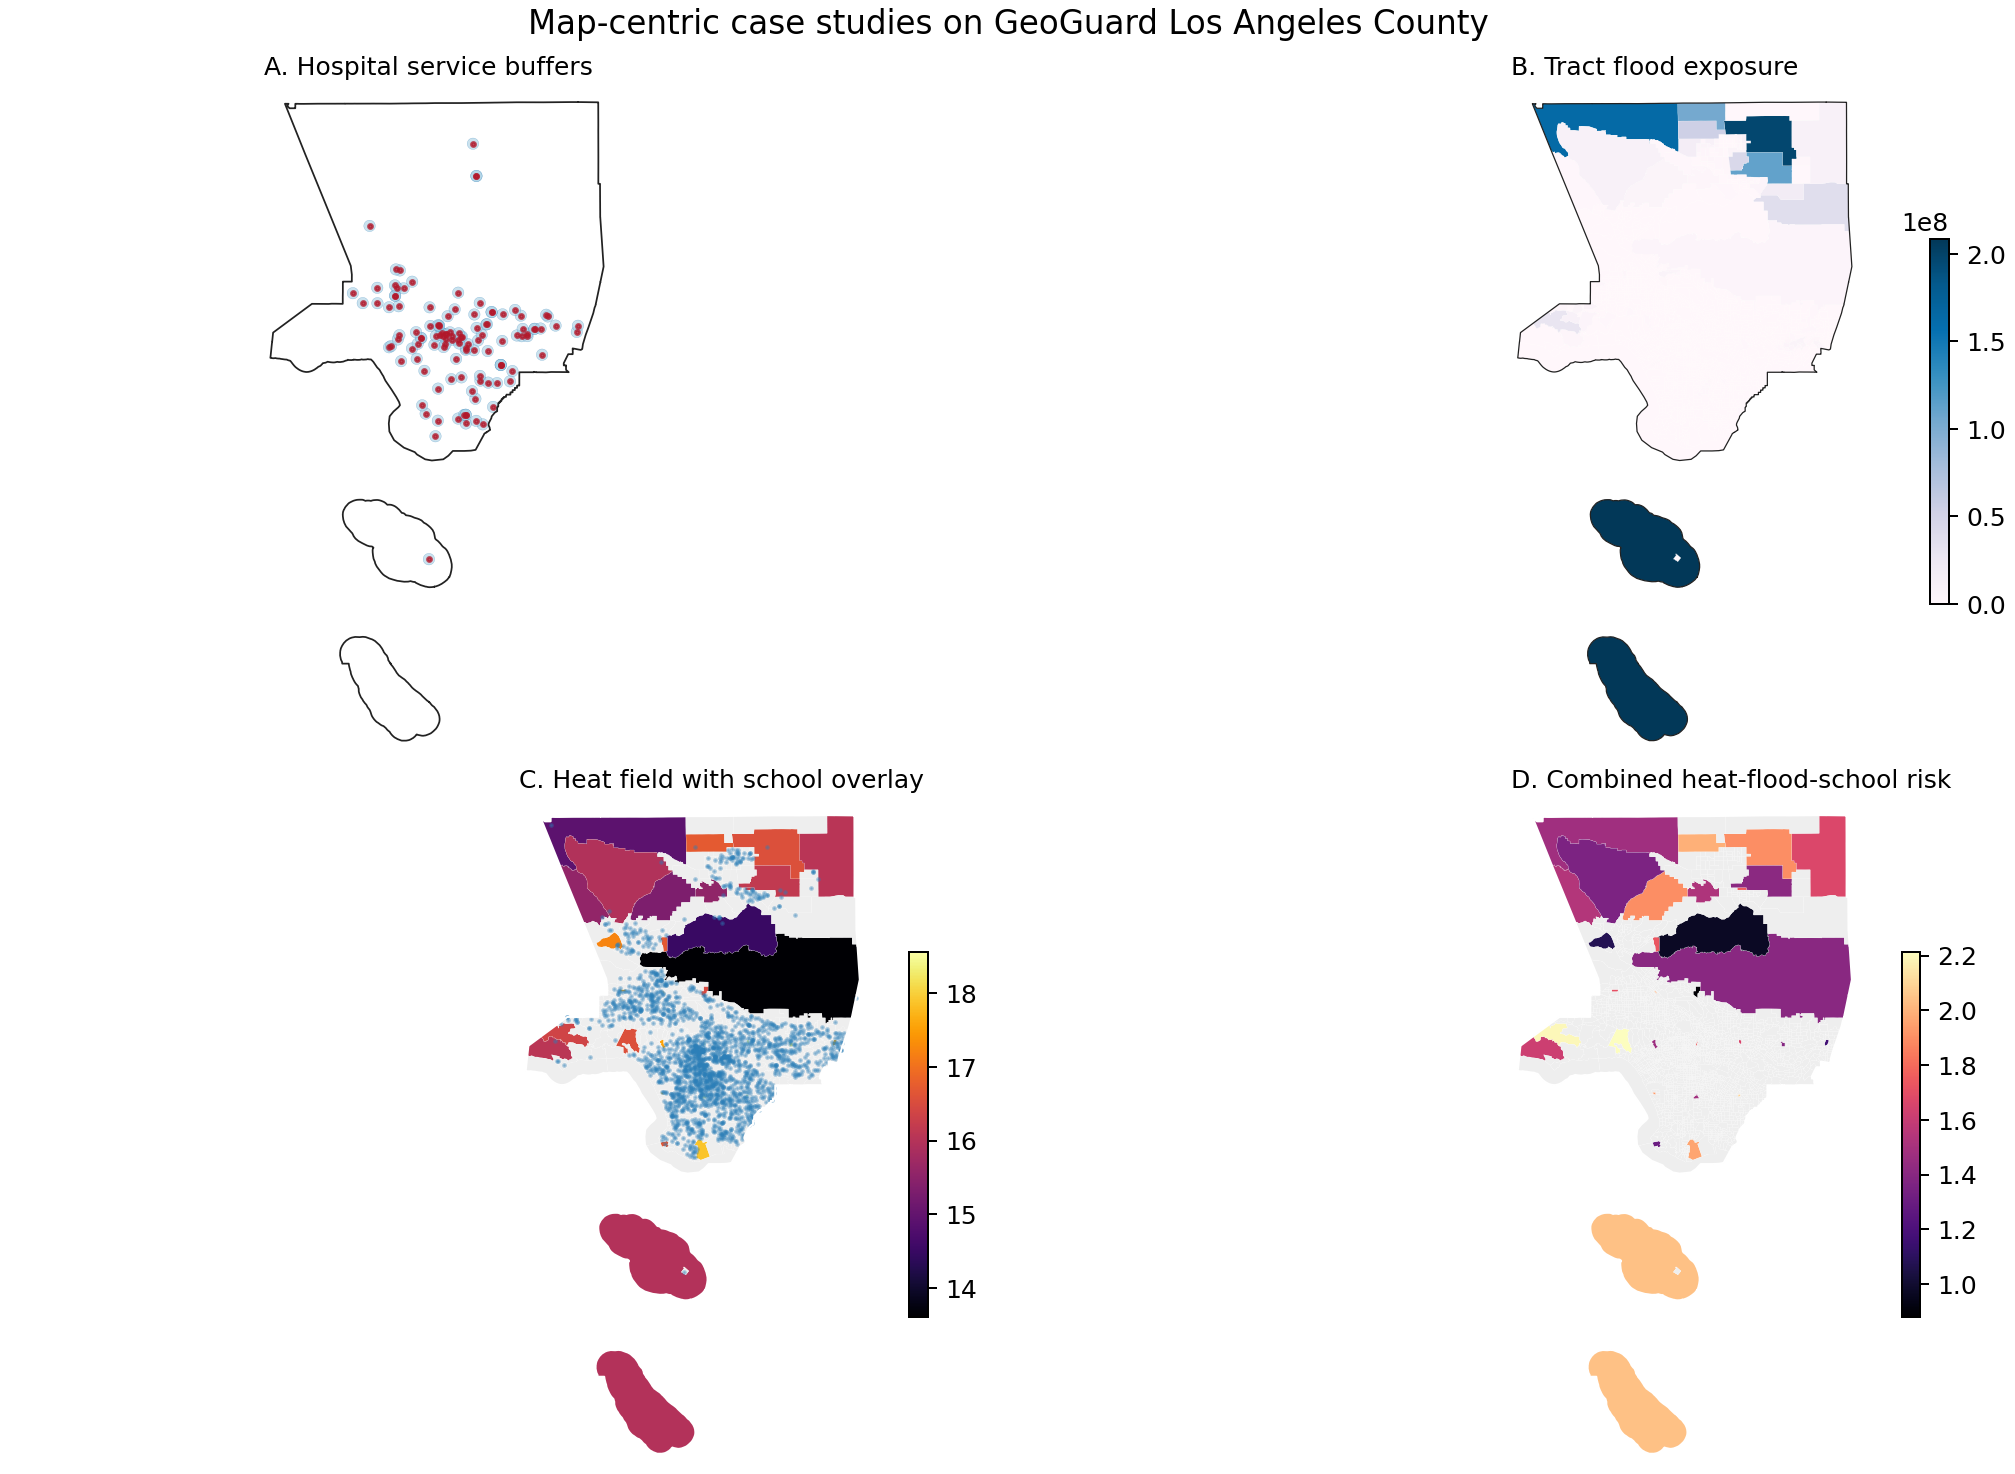
\includegraphics[width=0.96\textwidth]{figures/map_case_studies_geoguard.png}
\caption{Representative valid artifacts generated from GeoGuard contracts. The examples show that valid contracts produce concrete GIS outputs, including vector overlays, counted joins, raster-derived products, and map exports, rather than only passing textual validation.}
\label{fig:map-case-studies-geoguard}
\end{figure}

Finally, a mutation-based negative-control audit tests whether the validator detects known-bad contracts. Starting from 506 strict-valid base contracts, the audit injects 2165 controlled faults covering hallucinated layers, missing layer roles, wrong operation family, wrong output filename, invalid choropleth colormap, and unsafe metric-buffer CRS. Detection rates range from 0.943 for missing-layer-role mutations to 1.000 for wrong operation family, wrong output filename, invalid colormap, and unsafe metric-buffer CRS (Table~\ref{tab:negative-control}). This stress test does not prove completeness of the validator, but it provides direct evidence that the scorer detects the failure classes that motivate the benchmark.

\begin{table}[htbp]
\centering
\caption{Mutation-based negative-control audit over 2165 injected contract faults. Detection means the validator or execution adapter rejected the mutated contract for the intended failure reason.}
\label{tab:negative-control}
\small
\setlength{\tabcolsep}{4pt}
\begin{tabular}{lrrr}
\toprule
Mutation type & Cases & Detected & Rate \\
\midrule
Geographic CRS for metric buffer & 87 & 87 & 1.000 \\
Hallucinated layer alias & 506 & 502 & 0.992 \\
Invalid choropleth colormap & 54 & 54 & 1.000 \\
Missing required layer role & 506 & 477 & 0.943 \\
Wrong operation family & 506 & 506 & 1.000 \\
Wrong output filename & 506 & 506 & 1.000 \\
\bottomrule
\end{tabular}
\end{table}

\subsection{Failure patterns, model behavior, and task families}

Table~\ref{tab:failure-summary} and Figure~\ref{fig:failure-counts} show failure counts by mode. The contrast is starkest for data-invalid failures: basic mode produces 249 data-invalid rows out of 360, while grounded and GeoGuard modes produce only 31 and 25 respectively. This confirms that explicit data profiles are the main intervention against dataset hallucination. Field weakness remains more persistent: basic, grounded, and GeoGuard modes produce 168, 155, and 140 field-weak rows respectively. This indicates that knowing which layers exist does not automatically solve derived-field planning, aggregation fields, or output schema preservation. The table is used for exact counts; the figure emphasizes the relative collapse of data-invalid failures after grounding.

\begin{table}[htbp]
\centering
\caption{Failure counts by prompting mode. Counts are out of 360 task rows per mode.}
\label{tab:failure-summary}
\small
\setlength{\tabcolsep}{4pt}
\begin{tabular}{lrrrrrrrr}
\toprule
Mode & JSON & Tool & Data & Field & CRS & Schema & Map & Output \\
\midrule
Basic & 92 & 2 & 249 & 168 & 83 & 36 & 46 & 9 \\
Grounded & 55 & 8 & 31 & 155 & 89 & 45 & 10 & 19 \\
GeoGuard & 58 & 7 & 25 & 140 & 39 & 33 & 9 & 12 \\
\bottomrule
\end{tabular}
\end{table}

Table~\ref{tab:failure-summary} makes the same result visible as concrete error counts. Basic mode produces 249 data-invalid cases, which means that roughly two thirds of task rows reference unavailable or unsupported data. Grounded and GeoGuard modes reduce this failure class to 31 and 25, respectively, but field-weak cases remain high in all modes. This residual field problem is analytically important: it means that metadata grounding solves ``what layers exist'' better than it solves ``what attributes are preserved, generated, or aggregated.'' The table therefore motivates the later discussion of schema-transition contracts as a missing layer in LLM-GIS workflows.

\begin{figure}[htbp]
\centering
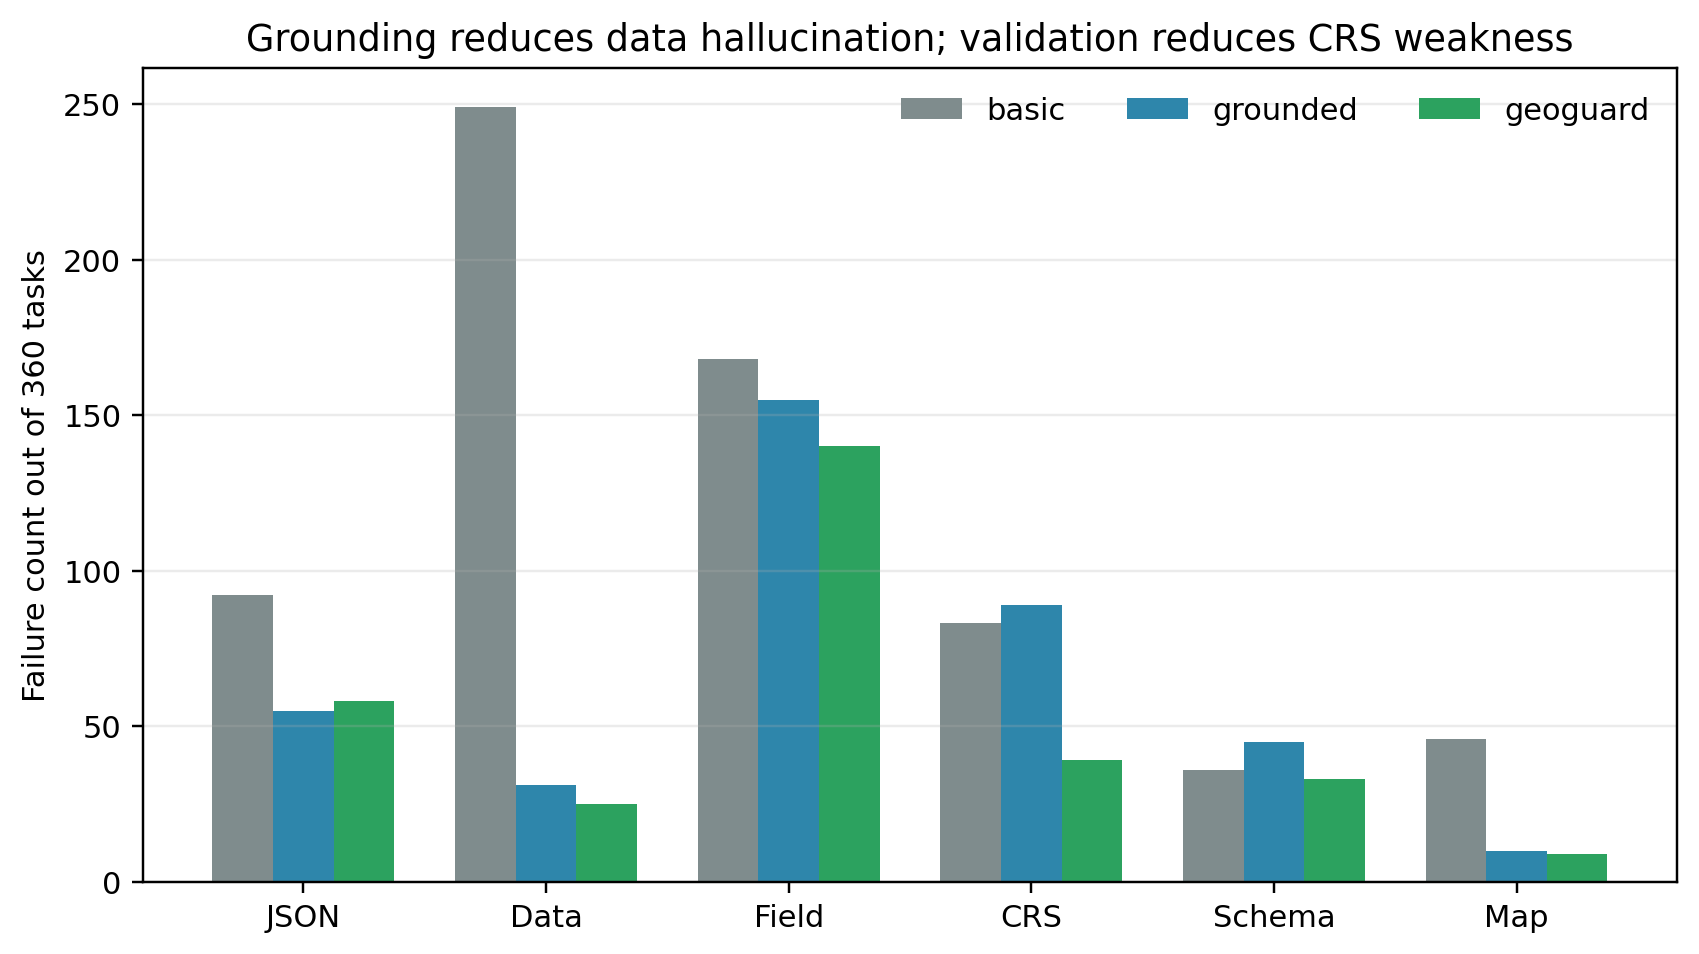
\includegraphics[width=0.92\textwidth]{figures/full_failure_counts_by_mode.png}
\caption{Failure counts across the full 30-task panel. Grounding sharply reduces data hallucination, while GeoGuard-style validation reduces CRS-weak planning. Field weakness remains the most persistent residual failure.}
\label{fig:failure-counts}
\end{figure}

The failure taxonomy also clarifies the distinct roles of grounding and validation. Grounding reduces data-invalid rows because the model no longer needs to guess which hospital, flood, tract, temperature, or map-input layers exist. GeoGuard reduces CRS-weak rows because it repeatedly states that metric buffers, area calculations, overlay operations, and raster masks require CRS alignment or projected coordinates. Neither intervention fully solves field weakness. The model must still know which school-count, hospital-count, flood-area, temperature-mean, and multivariate-risk fields are existing attributes and which are derived outputs created by a prior operation. Figure~\ref{fig:geo-failure-cases} grounds these abstract failure categories in map examples, showing why a format-valid workflow can still be geospatially unsafe.

\begin{figure}[htbp]
\centering
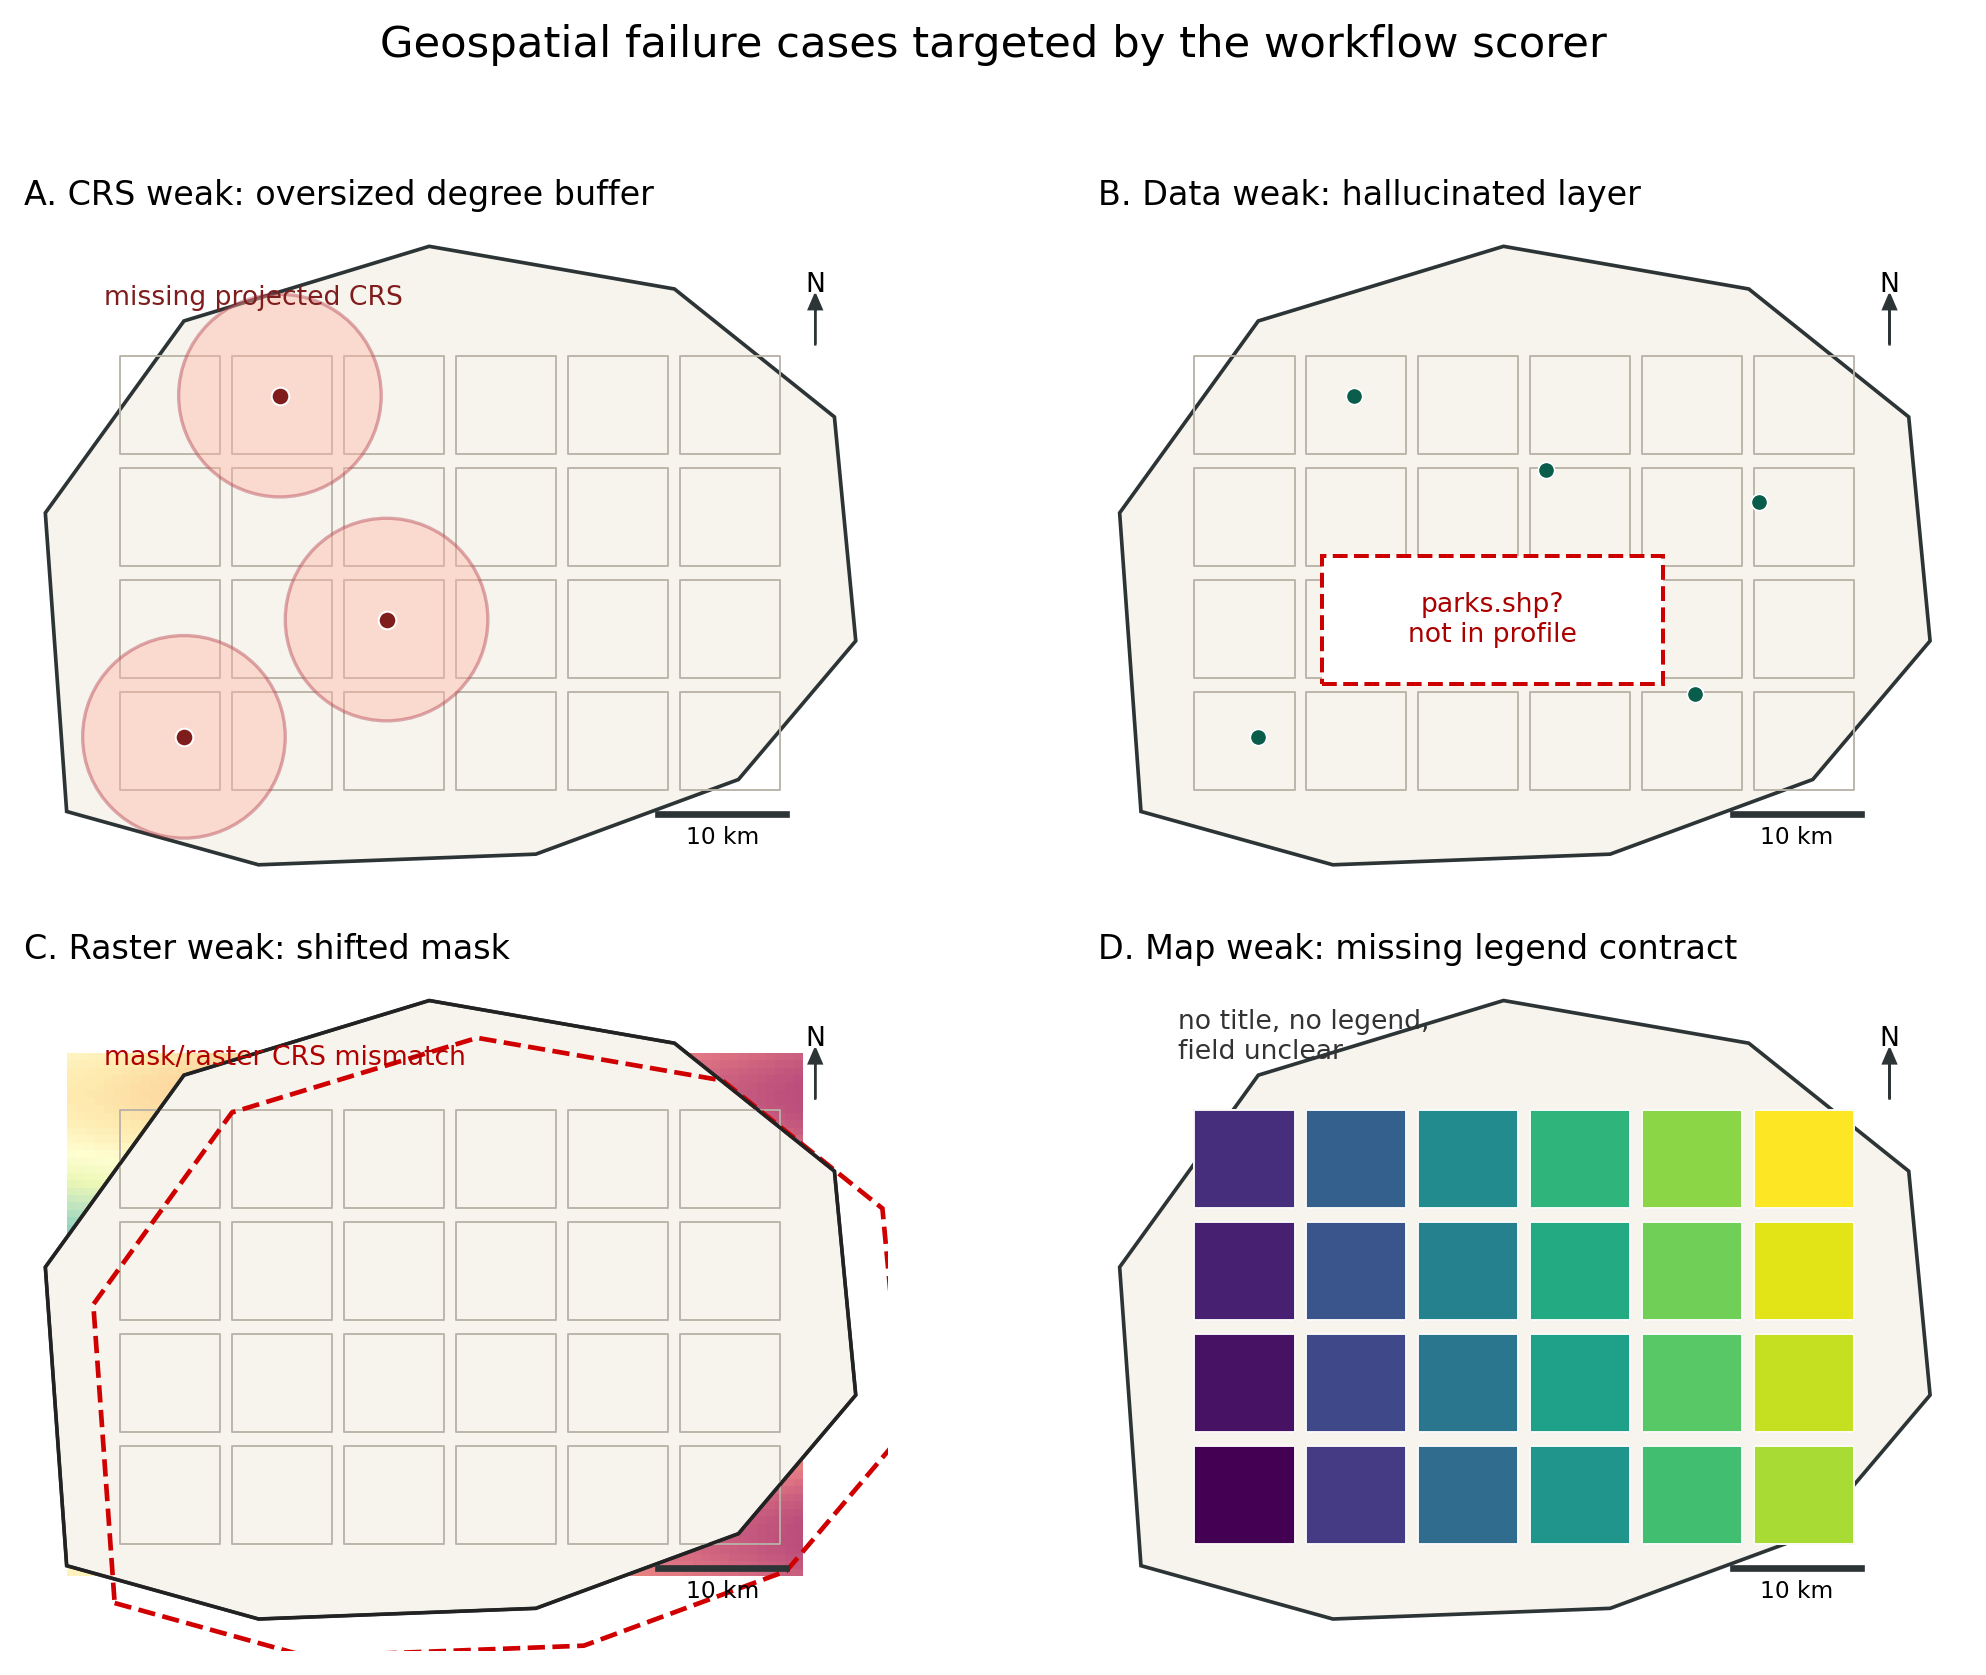
\includegraphics[width=0.78\textwidth]{figures/geo_failure_case_maps.png}
\caption{Representative geospatial failure cases targeted by the scorer. The benchmark treats missing projected CRS, hallucinated layers, shifted raster masks, and incomplete map contracts as distinct reliability failures rather than generic text-generation errors.}
\label{fig:geo-failure-cases}
\end{figure}

Table~\ref{tab:model-summary} and Figure~\ref{fig:model-heatmap} report model-level behavior. The strongest GeoGuard PRS values are achieved by qwen2.5-coder:3b (0.947), gemma3:4b (0.945), qwen2.5-coder:14b (0.938), qwen2.5-coder:7b (0.934), qwen2.5-coder:32b (0.934), deepseek-coder:6.7b (0.931), and qwen2.5-coder:1.5b (0.919). This result is important because it does not simply rank the largest model first. Small coder models and a compact general model can emit strong workflow specifications under a structured protocol, while qwen3:4b fails the strict JSON-contract protocol across the full panel. The table provides rankable numeric values, and the heatmap makes the mode sensitivity of each model visible at a glance.

\begin{table}[htbp]
\centering
\caption{Plan reliability score by model and mode in the full 30-task run.}
\label{tab:model-summary}
\small
\setlength{\tabcolsep}{4pt}
\begin{tabular}{lrrr}
\toprule
Model & Basic PRS & Grounded PRS & GeoGuard PRS \\
\midrule
deepseek-coder:6.7b & 0.610 & 0.902 & 0.931 \\
gemma3:4b & 0.773 & 0.911 & 0.945 \\
llama3.2:3b & 0.594 & 0.888 & 0.821 \\
mistral:7b & 0.539 & 0.765 & 0.823 \\
phi3:mini & 0.129 & 0.170 & 0.269 \\
qwen2.5-coder:1.5b & 0.551 & 0.902 & 0.919 \\
qwen2.5-coder:3b & 0.685 & 0.919 & 0.947 \\
qwen2.5-coder:7b & 0.698 & 0.880 & 0.934 \\
qwen2.5-coder:14b & 0.722 & 0.916 & 0.938 \\
qwen2.5-coder:32b & 0.681 & 0.915 & 0.934 \\
qwen2.5:3b & 0.579 & 0.841 & 0.823 \\
qwen3:4b & 0.000 & 0.000 & 0.000 \\
\bottomrule
\end{tabular}
\end{table}

Table~\ref{tab:model-summary} separates model compliance from model scale. The strongest GeoGuard results come from qwen2.5-coder:3b and gemma3:4b, while the larger qwen2.5-coder:32b is strong but not dominant. This suggests that the benchmark rewards structured-output discipline and geospatial contract following rather than parameter count alone. The table also shows two different failure regimes: qwen3:4b has a near-total contract failure under the prompt, whereas phi3:mini improves slightly but remains weak. These rows should not be read simply as ``bad GIS reasoning''; they indicate that some local models need a different structured-output interface before their geospatial reasoning can be evaluated fairly.

\begin{figure}[htbp]
\centering
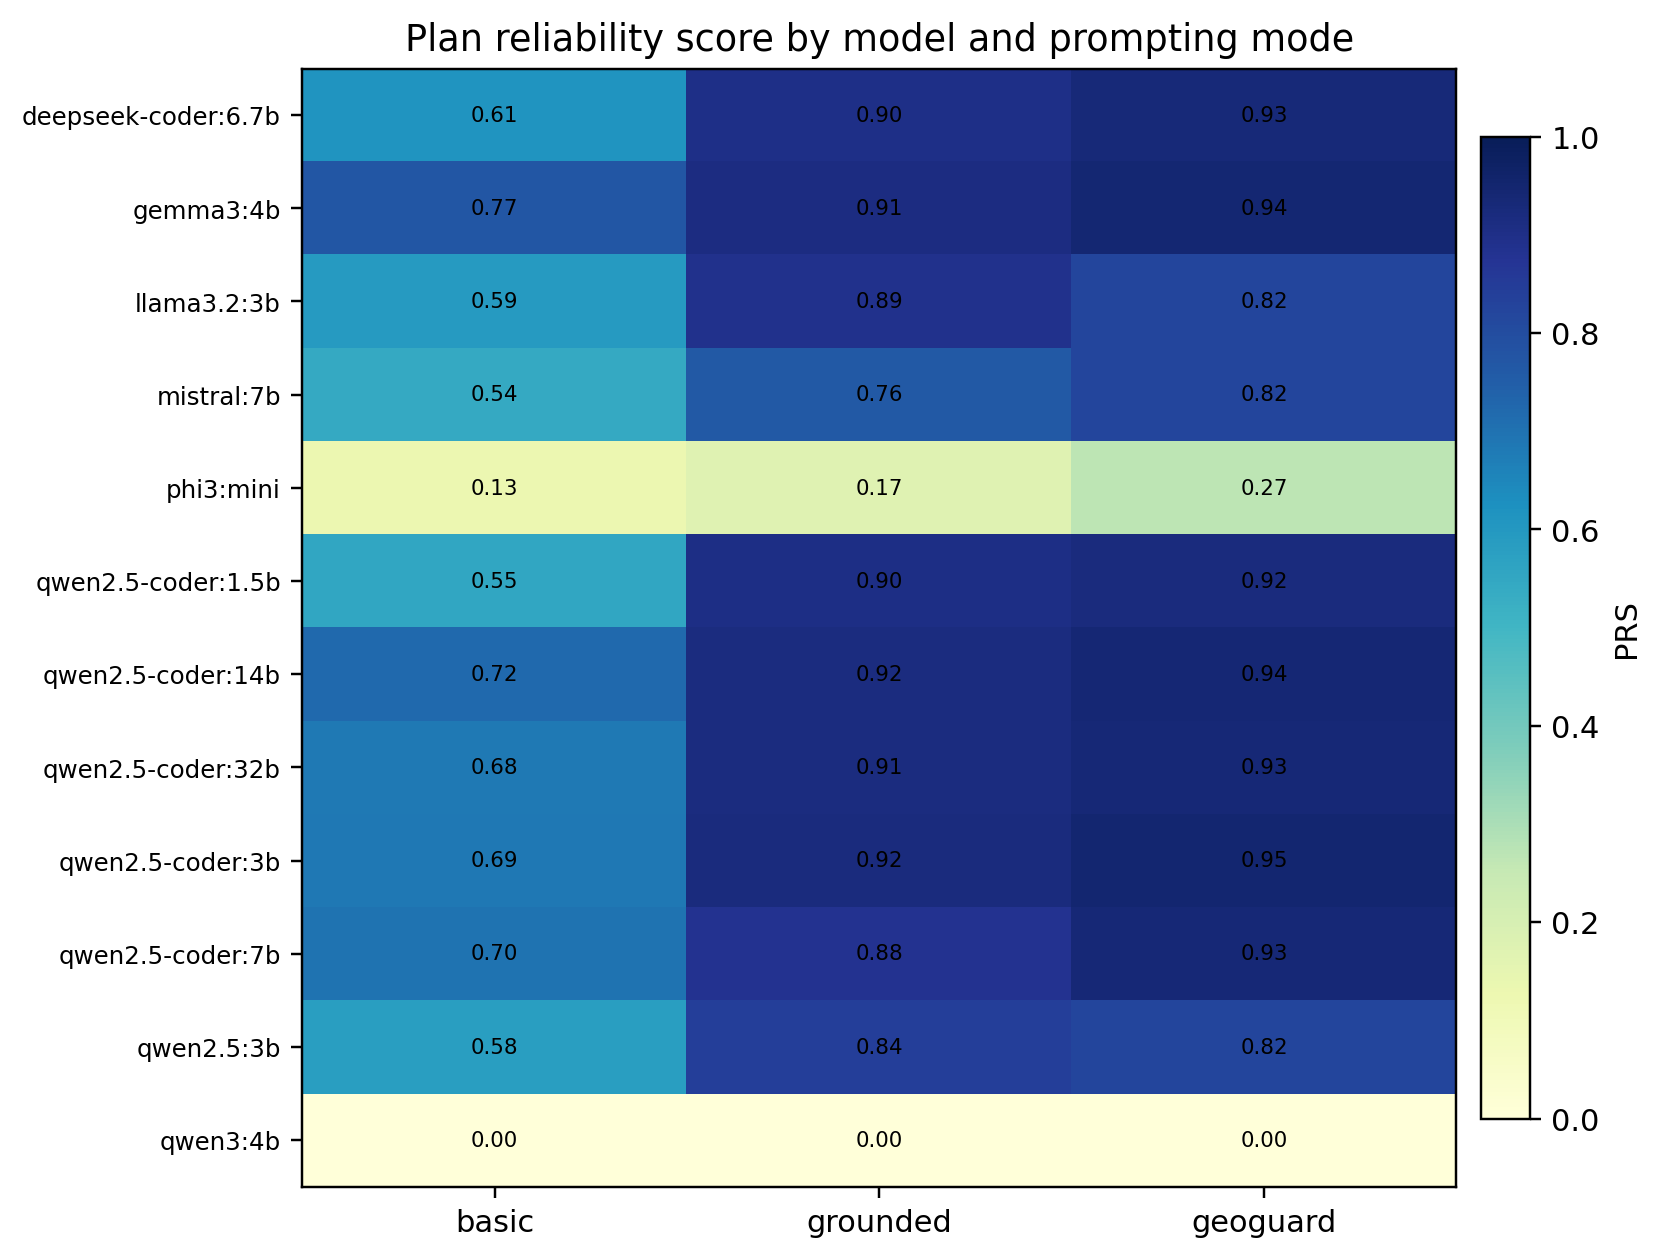
\includegraphics[width=0.78\textwidth]{figures/full_model_prs_heatmap.png}
\caption{Plan reliability score by model and prompting mode. The full panel shows that local structured workflow planning is not a simple function of model size: qwen2.5-coder:3b and gemma3:4b are among the strongest GeoGuard performers, while qwen3:4b fails the strict contract.}
\label{fig:model-heatmap}
\end{figure}

The model-level results separate three capabilities that are often collapsed in LLM-GIS discussion. First, a model must obey the output contract. Qwen3:4b and phi3:mini show that some local models are weak JSON-specification emitters under a uniform prompt even if they may be useful in conversational settings. Second, a model must ground itself in the known data profile. Basic-mode data validity is low for almost every model, including high-scoring basic performers such as gemma3:4b, because task-only prompts leave layer names underspecified. Third, a model must reason about geospatial validity. GeoGuard improves CRS planning for most contract-compliant models, but field validity remains a harder problem because derived schemas require more than recognizing input layers.

Figure~\ref{fig:category-prs} and Table~\ref{tab:category-summary} show that task families are not equally difficult. Basic-mode buffer tasks are the weakest family, with PRS 0.399, because the models often omit metric buffering and known layer references. GeoGuard lifts buffer PRS to 0.782. Raster clipping is the strongest family under GeoGuard, reaching PRS 0.845, because the validation rules directly match the required raster-mask CRS alignment. Point-count joins also benefit strongly, rising from 0.577 in basic mode to 0.820 in GeoGuard mode. The figure highlights family-level trends, while the table records the exact PRS values used in the comparison.

\begin{figure}[htbp]
\centering
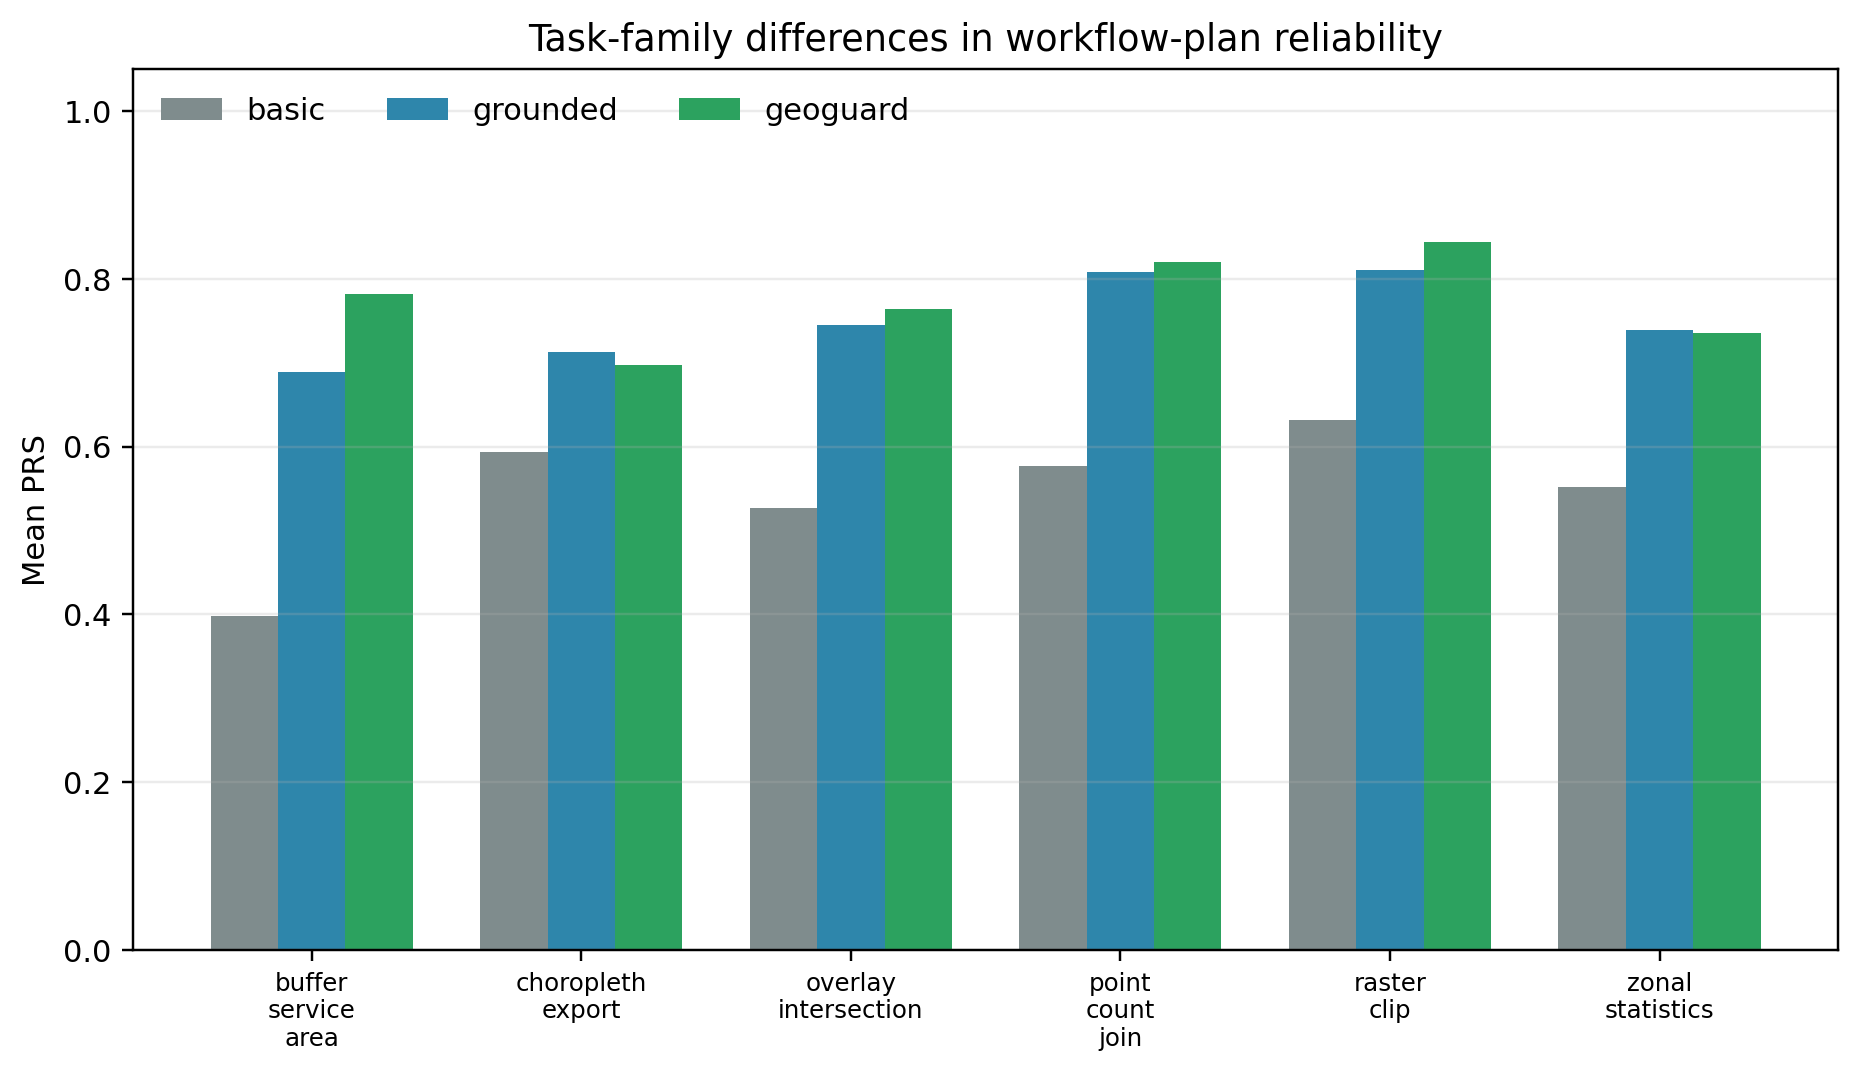
\includegraphics[width=0.95\textwidth]{figures/full_category_prs_by_mode.png}
\caption{Task-family plan reliability scores by prompting mode. Grounding and validation improve all task families, but the strongest gains differ: buffer and point-count tasks benefit sharply from GeoGuard rules, while choropleth export remains limited by field and map-plan weaknesses.}
\label{fig:category-prs}
\end{figure}

\begin{table}[htbp]
\centering
\caption{Plan reliability score by task family and prompting mode. Each cell summarizes 60 task rows.}
\label{tab:category-summary}
\small
\setlength{\tabcolsep}{4pt}
\begin{tabular}{lrrr}
\toprule
Task family & Basic PRS & Grounded PRS & GeoGuard PRS \\
\midrule
Buffer service area & 0.399 & 0.689 & 0.782 \\
Choropleth export & 0.594 & 0.712 & 0.697 \\
Overlay intersection & 0.527 & 0.746 & 0.764 \\
Point-count join & 0.577 & 0.808 & 0.820 \\
Raster clip & 0.632 & 0.811 & 0.845 \\
Zonal statistics & 0.552 & 0.739 & 0.735 \\
\bottomrule
\end{tabular}
\end{table}

Table~\ref{tab:category-summary} shows that task family is a major source of variance. Raster clip is the strongest GeoGuard family because its central requirement, raster-mask CRS alignment, is directly named by the validation rules. Buffer tasks show the largest relative improvement because metric CRS guidance corrects a common basic-mode weakness. Choropleth export is the exception: GeoGuard does not outperform grounded prompting because map export depends on thematic-field choice and cartographic design, not only on geospatial validity checks. This family-level pattern argues that GIS copilots need separate validation modules for spatial analysis and map communication.

Choropleth export behaves differently. Grounded mode slightly outperforms GeoGuard in PRS, 0.712 versus 0.697, because GeoGuard introduces more validation context without fully solving the harder question of which derived field a map should use. In this family, map plan improves relative to basic mode, but field validity remains weak. This result is cartographically important. A workflow can name the correct data layer and still fail to state a defensible thematic field, classification scheme, or legend contract. Map production therefore needs a cartographic design contract in addition to GIS validity rules. Figure~\ref{fig:geo-cartographic-variants} illustrates this distinction: the same tract geometry can be a weak map, a grounded thematic map, or a publication-ready export depending on whether the workflow contract includes cartographic elements.

\begin{figure}[htbp]
\centering
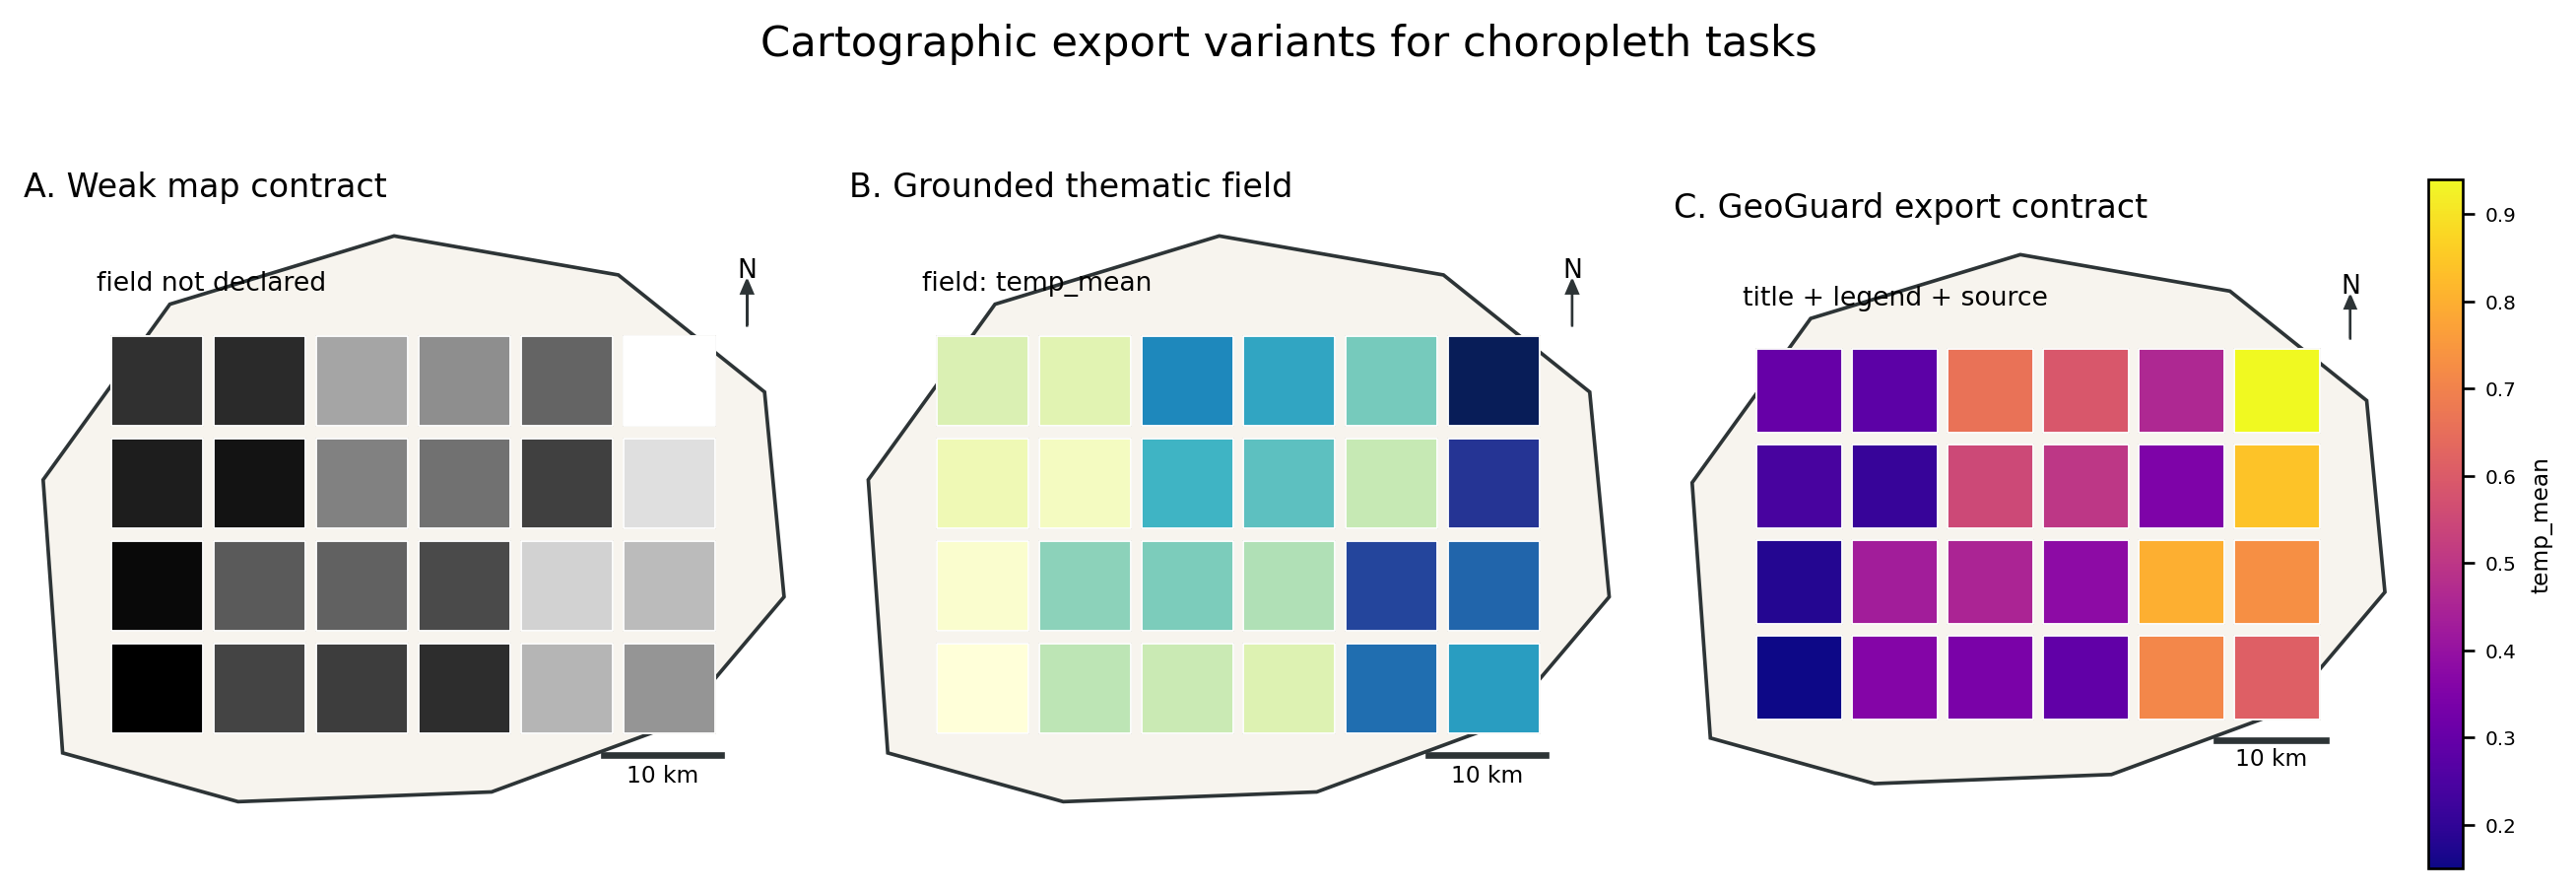
\includegraphics[width=0.98\textwidth]{figures/geo_cartographic_export_variants.png}
\caption{Cartographic export variants for choropleth tasks. The map family requires more than a valid layer reference: the workflow contract must identify a thematic field, classification or color strategy, title, legend, and source-note requirements.}
\label{fig:geo-cartographic-variants}
\end{figure}

\section{Discussion}

\subsection{Workflow-contract interpretation}

The full experiment supports the premise that workflow specifications are a useful evaluation layer for Geo-LLM systems. In a GIS setting, the model output is not merely text that precedes code; it is a proposed spatial procedure with commitments about layers, fields, CRS transformations, predicates, schemas, and cartographic outputs. Making those commitments explicit turns an opaque natural-language interaction into a testable interface object. This mirrors a systems tradition in geoinformatics: spatial objects, outlier definitions, route queries, and surface-generation procedures become reliable when the task representation and validity conditions are formalized before application deployment \citep{Shekhar_1999_ObjectDirection,Shekhar_2003_SpatialOutliers,Yoo_2005_InRouteNN,Camelli_2012_SeamlessSurfaces}.

The benchmark also changes where failures can be diagnosed. If a model cannot name the correct input layers, preserve required fields, or state a CRS strategy for a buffer, overlay, raster mask, or zonal statistic, downstream code generation is unlikely to be trustworthy. Conversely, a valid specification can be inspected, repaired, or executed by deterministic tooling. This is not a replacement for code execution or map-quality review. It is a preceding layer that makes later failures easier to attribute: the executor, the data binding, the numerical result, and the cartographic representation can be assessed after the spatial plan has been made explicit.

\subsection{Grounding, validation, and task-family implications}

The difference between grounded and GeoGuard modes is instructive. Grounding largely solves dataset hallucination by telling models what layers and operations exist. Validation rules mainly improve CRS planning. This result complements geospatial code-generation and autonomous-GIS work, which shows that LLMs can generate GIS code or geoprocessing workflows but still need structured operation knowledge and execution constraints \citep{Hou_2025_GeoCode,Hou_2025_GEEOPs,Li_2025_AutonomousGIS}. Data profiles answer the question ``what exists?'' Tool schemas answer ``what can be done?'' Validation rules answer ``what must be true for the operation to be spatially valid?'' A robust copilot architecture should provide all three.

The residual field-validity problem is a different kind of error. It is not enough for the model to know that a layer exists. It must also know when a field is an input attribute, when it is an output attribute created by an operation, and when it is a derived design variable that requires a previous analysis step. This explains why field weakness remains high even after grounding and validation. The benchmark therefore suggests a fourth context layer for future GIS copilots: an explicit schema-transition contract that describes which fields are preserved, generated, aggregated, or consumed by each operation.

The six task families diagnose different parts of the GIS-copilot stack. Buffer tasks stress measurement units and projected CRS selection. Overlay tasks stress multi-layer alignment and output-field preservation. Point-count joins stress spatial predicates and generated count fields. Raster clips stress raster-vector CRS alignment and nodata handling. Zonal statistics stress raster-vector interaction plus derived statistical fields. Choropleth export stresses cartographic communication rather than spatial analysis alone.

This decomposition matters because a single average score can hide very different failure modes. Raster clipping has the highest GeoGuard PRS because the validation rule directly matches the operation's central risk: align the mask to the raster CRS before clipping. Choropleth export remains weaker because the operation is underspecified if the model has to choose a thematic field, classification, color ramp, title, legend, and source note from a derived or ambiguous layer. These cartographic choices are not solved by a generic CRS validator. They require a map-design contract that is closer to cartographic specification and visualization-quality guidance than to ordinary GIS preprocessing \citep{Roth_2013,Roth_2015,Kang_2024,Munzner_2009}.

The experiment was intentionally restricted to locally installed Ollama models. This choice matters for reproducibility and cost: all generations can be rerun without cloud APIs, rate limits, or proprietary model access. It also reveals the heterogeneity of local models. Some compact models are not suitable for strict JSON workflow planning under the present prompt. Others, including small coder models, perform strongly across the full 30-task panel when grounded and constrained.

The model rankings should still be read as workflow-contract rankings rather than universal LLM rankings. The benchmark rewards models that emit strict JSON, name known layers, declare required fields, and state validation checks. A model that fails this protocol may still be useful with a different prompting interface or a native structured-output API. Conversely, a high workflow-specification score does not prove that the generated specification will execute successfully or produce a publication-quality map. It shows that the plan is structured enough for the next layer of deterministic execution and artifact validation.

The strongest practical finding is that smaller local models can be competitive when the task is framed as structured planning rather than free-form code generation. Qwen2.5-coder:3b and gemma3:4b are among the strongest GeoGuard performers, and qwen2.5-coder:1.5b remains above 0.91 PRS. This matters for reproducible GIS-assistant research because local inference avoids proprietary APIs, rate limits, and model-version drift. The result does not imply that these models can replace stronger cloud models for open-ended GIS coding. It shows that a constrained workflow-contract interface can make local models useful for a narrower but operationally important planning role.

\subsection{Limitations and next steps}

This study reports the full planning sweep, a post-scoring execution-readiness gate, deterministic full-cohort execution, bounded role-default repair, and a mutation-based negative-control audit. The evidence covers twelve models, three modes, and 30 tasks, yielding 1080 attempted specifications. The execution analysis is still an initial runtime layer: it tests whether workflow contracts can be bound to deterministic GIS operations and produce valid artifacts, but it does not yet evaluate every numerical output against an expert-curated reference result or every map against a human cartographic-quality rubric.

The current scorer is rule-based. It checks explicit layer names, field references, CRS signals, schema declarations, map-plan tokens, and output filenames. This is appropriate for a reproducible first pass and is supported by the negative-control audit, but it cannot assess every plausible workflow representation. Future versions should add richer operation-specific parameter validation, compare artifact-level results with numerical reference outputs, and include independent expert review of cartographic quality.

The benchmark also uses a single prompt template per mode. Some models, especially qwen3:4b and phi3:mini, may improve with model-specific format controls. This paper deliberately avoids per-model prompt tuning because the goal is a uniform contract. A later robustness analysis can compare uniform prompting with model-specific structured-output prompting.

Finally, the current benchmark uses synthetic but realistic task contracts over a fixed data profile. This is appropriate for isolating planning behavior, but it does not cover the full diversity of GIS practice. Future task sets should include temporal joins, network analysis, raster resampling, uncertainty propagation, scale-dependent cartographic generalization, and interactive web-map export. They should also include adversarial prompts that intentionally mention unavailable layers or ambiguous fields, because real users often phrase GIS requests with incomplete data knowledge.

\paragraph{Integrated full-run ledgers.}

The following tables record the main full-run ledgers inside the manuscript so the paper can be read without opening external experiment files. The complete machine-readable ledgers remain in the archived package and should be treated as the reproducibility source of record. Table~\ref{tab:model-mode-full} gives the complete model-by-mode metric profile, and Table~\ref{tab:failure-family-full} gives the corresponding family-level failure counts.

\begin{table}[htbp]
\centering
\caption{Full model-by-mode reliability metrics.}
\label{tab:model-mode-full}
\small
\setlength{\tabcolsep}{3pt}
\begin{tabular}{llrrrrrr}
\toprule
Model & Mode & JSON & Data & Field & CRS & WPHR & PRS \\
\midrule
deepseek-coder:6.7b & Basic & 0.800 & 0.067 & 0.372 & 0.633 & 0.479 & 0.610 \\
deepseek-coder:6.7b & Grounded & 1.000 & 0.867 & 0.646 & 0.783 & 0.141 & 0.902 \\
deepseek-coder:6.7b & GeoGuard & 1.000 & 0.900 & 0.682 & 0.933 & 0.097 & 0.931 \\
gemma3:4b & Basic & 1.000 & 0.133 & 0.586 & 0.833 & 0.320 & 0.773 \\
gemma3:4b & Grounded & 1.000 & 1.000 & 0.690 & 0.750 & 0.123 & 0.911 \\
gemma3:4b & GeoGuard & 1.000 & 0.967 & 0.817 & 0.867 & 0.077 & 0.945 \\
llama3.2:3b & Basic & 0.867 & 0.067 & 0.178 & 0.567 & 0.524 & 0.594 \\
llama3.2:3b & Grounded & 0.967 & 0.967 & 0.760 & 0.883 & 0.120 & 0.888 \\
llama3.2:3b & GeoGuard & 0.900 & 0.900 & 0.547 & 0.817 & 0.194 & 0.821 \\
mistral:7b & Basic & 0.800 & 0.067 & 0.244 & 0.700 & 0.536 & 0.539 \\
mistral:7b & Grounded & 1.000 & 0.867 & 0.390 & 0.750 & 0.215 & 0.765 \\
mistral:7b & GeoGuard & 0.967 & 0.867 & 0.463 & 0.917 & 0.164 & 0.823 \\
phi3:mini & Basic & 0.200 & 0.000 & 0.067 & 0.200 & 0.903 & 0.129 \\
phi3:mini & Grounded & 0.267 & 0.200 & 0.133 & 0.200 & 0.827 & 0.170 \\
phi3:mini & GeoGuard & 0.300 & 0.300 & 0.180 & 0.300 & 0.713 & 0.269 \\
qwen2.5:3b & Basic & 0.833 & 0.000 & 0.244 & 0.650 & 0.520 & 0.579 \\
qwen2.5:3b & Grounded & 1.000 & 0.633 & 0.564 & 0.817 & 0.222 & 0.841 \\
qwen2.5:3b & GeoGuard & 0.933 & 0.667 & 0.488 & 0.750 & 0.221 & 0.823 \\
qwen2.5-coder:1.5b & Basic & 0.767 & 0.100 & 0.322 & 0.333 & 0.587 & 0.551 \\
qwen2.5-coder:1.5b & Grounded & 1.000 & 0.867 & 0.832 & 0.750 & 0.143 & 0.902 \\
qwen2.5-coder:1.5b & GeoGuard & 1.000 & 0.800 & 0.878 & 0.967 & 0.107 & 0.919 \\
qwen2.5-coder:3b & Basic & 0.900 & 0.067 & 0.378 & 0.733 & 0.404 & 0.685 \\
qwen2.5-coder:3b & Grounded & 1.000 & 0.967 & 0.694 & 0.750 & 0.118 & 0.919 \\
qwen2.5-coder:3b & GeoGuard & 1.000 & 0.967 & 0.788 & 0.867 & 0.076 & 0.947 \\
qwen2.5-coder:7b & Basic & 0.933 & 0.000 & 0.378 & 0.733 & 0.404 & 0.698 \\
qwen2.5-coder:7b & Grounded & 0.967 & 0.867 & 0.836 & 0.783 & 0.150 & 0.880 \\
qwen2.5-coder:7b & GeoGuard & 1.000 & 0.900 & 0.861 & 0.983 & 0.085 & 0.934 \\
qwen2.5-coder:14b & Basic & 0.933 & 0.067 & 0.411 & 0.767 & 0.369 & 0.722 \\
qwen2.5-coder:14b & Grounded & 0.967 & 0.967 & 0.817 & 0.783 & 0.107 & 0.916 \\
qwen2.5-coder:14b & GeoGuard & 0.967 & 0.967 & 0.816 & 0.917 & 0.082 & 0.938 \\
qwen2.5-coder:32b & Basic & 0.900 & 0.067 & 0.354 & 0.683 & 0.419 & 0.681 \\
qwen2.5-coder:32b & Grounded & 1.000 & 0.933 & 0.810 & 0.833 & 0.111 & 0.915 \\
qwen2.5-coder:32b & GeoGuard & 1.000 & 1.000 & 0.842 & 0.967 & 0.078 & 0.934 \\
qwen3:4b & Basic & 0.000 & 0.000 & 0.000 & 0.000 & 1.000 & 0.000 \\
qwen3:4b & Grounded & 0.000 & 0.000 & 0.000 & 0.000 & 1.000 & 0.000 \\
qwen3:4b & GeoGuard & 0.000 & 0.000 & 0.000 & 0.000 & 1.000 & 0.000 \\
\bottomrule
\end{tabular}
\end{table}

Table~\ref{tab:model-mode-full} is useful for audit because it preserves secondary metrics that are compressed in the main model summary, including JSON validity, data validity, field validity, CRS planning, and weighted hallucination risk. It shows, for example, that several strong GeoGuard models still differ in field validity even when their aggregate PRS values are close. The table also reveals why PRS alone should not be treated as the only ranking criterion: qwen2.5-coder:7b and qwen2.5-coder:32b have similar GeoGuard PRS values, but they arrive there through different field-validity and CRS-planning profiles. For a deployed GIS copilot, this distinction matters because a workflow that is CRS-safe but field-weak will fail differently from one that preserves schema but omits a projection strategy.

\begin{table}[htbp]
\centering
\caption{Failure counts by task family and prompting mode. Counts are out of 60 rows per family-mode pair.}
\label{tab:failure-family-full}
\small
\setlength{\tabcolsep}{3pt}
\begin{tabular}{llrrrrrr}
\toprule
Task family & Mode & JSON & Data & Field & CRS & Map & Output \\
\midrule
Buffer & Basic & 24 & 35 & 32 & 52 & 0 & 5 \\
Buffer & Grounded & 12 & 4 & 17 & 48 & 0 & 7 \\
Buffer & GeoGuard & 11 & 1 & 10 & 19 & 0 & 2 \\
Choropleth & Basic & 14 & 46 & 3 & 0 & 46 & 1 \\
Choropleth & Grounded & 10 & 11 & 11 & 0 & 10 & 2 \\
Choropleth & GeoGuard & 12 & 8 & 14 & 0 & 9 & 4 \\
Overlay & Basic & 13 & 43 & 56 & 25 & 0 & 1 \\
Overlay & Grounded & 6 & 7 & 34 & 31 & 0 & 4 \\
Overlay & GeoGuard & 10 & 4 & 24 & 26 & 0 & 2 \\
Point-count & Basic & 11 & 49 & 50 & 16 & 0 & 1 \\
Point-count & Grounded & 7 & 4 & 34 & 7 & 0 & 3 \\
Point-count & GeoGuard & 6 & 4 & 25 & 6 & 0 & 1 \\
Raster & Basic & 17 & 37 & 0 & 22 & 0 & 0 \\
Raster & Grounded & 10 & 5 & 0 & 10 & 0 & 0 \\
Raster & GeoGuard & 8 & 7 & 0 & 8 & 0 & 0 \\
Zonal & Basic & 13 & 39 & 27 & 20 & 0 & 1 \\
Zonal & Grounded & 10 & 0 & 59 & 0 & 0 & 3 \\
Zonal & GeoGuard & 11 & 1 & 57 & 0 & 0 & 3 \\
\bottomrule
\end{tabular}
\end{table}

Table~\ref{tab:failure-family-full} shows which failure categories dominate each task family. Buffer tasks concentrate CRS weaknesses, choropleth tasks concentrate map-plan weaknesses, and zonal tasks concentrate field/schema weaknesses, matching the diagnostic interpretation in the main results. The family-mode breakdown is useful because it prevents an overly broad conclusion such as ``GeoGuard fixes GIS errors.'' It does not. GeoGuard sharply reduces CRS-weak buffer cases, but it leaves many zonal field-weak cases unresolved and only modestly improves choropleth map-plan failures. The table therefore identifies where additional experiment design is needed: schema-transition rules for zonal/aggregation tasks and explicit cartographic contracts for export tasks.

\paragraph{Compact task and hard-case ledgers.}

The previous tables summarize the full run at model and family levels. The following compact ledgers make the experimental basis explicit without printing every generated row. Table~\ref{tab:task-suite-summary} summarizes the complete 30-task suite without listing task-level filenames, Table~\ref{tab:task-prs-matrix} gives a task-level PRS matrix across modes, Table~\ref{tab:geoguard-model-family-matrix} gives a GeoGuard model-by-family matrix, and Table~\ref{tab:geoguard-hard-cases} lists the lowest-scoring GeoGuard task-model cases after removing malformed JSON responses. The complete machine-readable ledgers, including all 1080 task-level rows and the full category-by-model-by-mode summaries, remain in the archived package and are the reproducibility source of record.

\begin{table}[htbp]
\centering
\caption{Task-suite summary by operation family. The table reports the reproducible contract dimensions without listing per-task artifact filenames.}
\label{tab:task-suite-summary}
\small
\begin{tabular}{p{0.19\textwidth}rp{0.28\textwidth}p{0.36\textwidth}}
\toprule
Task family & Tasks & Main contract focus & Required output information \\
\midrule
Buffer service area & 5 & metric distance and clipping & geometry plus retained or derived attributes \\
Overlay intersection & 5 & polygon interaction and area & tract identifier and flood attributes \\
Point-count join & 5 & point-in-polygon aggregation & tract identifier and generated count fields \\
Raster clip & 5 & raster-mask alignment & georeferenced raster output metadata \\
Zonal statistics & 5 & raster-vector summaries & tract identifier and derived temperature fields \\
Choropleth export & 5 & thematic map communication & thematic field, legend, title, classification, and source note \\
\bottomrule
\end{tabular}
\end{table}

Table~\ref{tab:task-suite-summary} is included to make clear which contract dimensions the benchmark expects. It is a task-suite summary rather than a performance table: each row defines the operation family, main validation focus, and required output information against which model responses are scored. The sequence of tasks also explains why the benchmark is harder than a one-operation demo: early tasks test buffers and overlays, middle tasks require generated count or area fields, and later tasks require raster-derived fields and cartographic exports. The table is therefore part of the integrated method-and-results evidence, not supplementary decoration.

\clearpage

\begin{table}[H]
\centering
\caption{Compact task-level PRS matrix across prompting modes. Each cell averages twelve local models.}
\label{tab:task-prs-matrix}
\small
\setlength{\tabcolsep}{4pt}
\begin{tabular}{llrrrr}
\toprule
Task & Family & Basic & Grounded & GeoGuard & Gain \\
\midrule
T001 & Buffer & 0.465 & 0.713 & 0.748 & 0.283 \\
T002 & Buffer & 0.322 & 0.726 & 0.811 & 0.489 \\
T003 & Buffer & 0.561 & 0.722 & 0.739 & 0.178 \\
T004 & Buffer & 0.291 & 0.691 & 0.800 & 0.509 \\
T005 & Buffer & 0.354 & 0.591 & 0.813 & 0.459 \\
T006 & Overlay & 0.491 & 0.769 & 0.778 & 0.287 \\
T007 & Overlay & 0.541 & 0.721 & 0.840 & 0.299 \\
T008 & Overlay & 0.537 & 0.800 & 0.776 & 0.239 \\
T009 & Overlay & 0.528 & 0.716 & 0.672 & 0.144 \\
T010 & Overlay & 0.537 & 0.722 & 0.753 & 0.216 \\
T011 & Point count & 0.612 & 0.877 & 0.868 & 0.256 \\
T012 & Point count & 0.650 & 0.834 & 0.831 & 0.181 \\
T013 & Point count & 0.530 & 0.750 & 0.748 & 0.218 \\
T014 & Point count & 0.567 & 0.843 & 0.851 & 0.284 \\
T015 & Point count & 0.526 & 0.735 & 0.801 & 0.275 \\
T016 & Raster & 0.722 & 0.800 & 0.800 & 0.078 \\
T017 & Raster & 0.650 & 0.811 & 0.894 & 0.244 \\
T018 & Raster & 0.633 & 0.822 & 0.822 & 0.189 \\
T019 & Raster & 0.567 & 0.800 & 0.883 & 0.317 \\
T020 & Raster & 0.589 & 0.822 & 0.822 & 0.233 \\
T021 & Zonal & 0.611 & 0.752 & 0.793 & 0.181 \\
T022 & Zonal & 0.502 & 0.780 & 0.780 & 0.278 \\
T023 & Zonal & 0.506 & 0.754 & 0.678 & 0.173 \\
T024 & Zonal & 0.580 & 0.725 & 0.715 & 0.136 \\
T025 & Zonal & 0.561 & 0.685 & 0.709 & 0.148 \\
T026 & Choropleth & 0.676 & 0.769 & 0.694 & 0.019 \\
T027 & Choropleth & 0.644 & 0.698 & 0.684 & 0.040 \\
T028 & Choropleth & 0.600 & 0.781 & 0.809 & 0.209 \\
T029 & Choropleth & 0.728 & 0.654 & 0.617 & -0.111 \\
T030 & Choropleth & 0.322 & 0.659 & 0.681 & 0.359 \\
\bottomrule
\end{tabular}
\end{table}


Table~\ref{tab:task-prs-matrix} condenses 1080 task-level rows into one row per task, so it is the most direct task-level diagnostic table in the manuscript. The gain column shows that the benchmark is not driven by a single easy family: buffer, overlay, point-count, raster, zonal, and choropleth tasks all contain cases where grounding or validation improves PRS. The largest gains occur when the basic prompt leaves layer identity, CRS handling, or derived output fields implicit, such as buffer and map-export tasks that require a concrete artifact contract. The smaller gains are also informative. They appear in tasks where the model already has enough spatial context or where metadata does not fully determine the cartographic decision. The negative gain in one choropleth case is especially useful because it shows that adding validation context can distract from thematic-field and map-design selection. Reading the table by row therefore helps identify which future tasks need richer contracts rather than merely stronger models.

\begin{table}[H]
\centering
\caption{Compact GeoGuard PRS matrix by model and GIS task family.}
\label{tab:geoguard-model-family-matrix}
\small
\setlength{\tabcolsep}{3pt}
\begin{tabular}{lrrrrrrr}
\toprule
Model & Buffer & Overlay & Points & Raster & Zonal & Choro. & Mean \\
\midrule
deepseek-coder:6.7b & 1.000 & 0.898 & 0.977 & 0.973 & 0.898 & 0.840 & 0.931 \\
gemma3:4b & 0.947 & 0.878 & 0.925 & 1.000 & 0.918 & 1.000 & 0.945 \\
llama3.2:3b & 0.898 & 0.744 & 0.815 & 1.000 & 0.747 & 0.720 & 0.821 \\
mistral:7b & 0.902 & 0.891 & 0.760 & 0.947 & 0.524 & 0.916 & 0.823 \\
phi3:mini & 0.000 & 0.191 & 0.633 & 0.400 & 0.191 & 0.200 & 0.269 \\
qwen2.5-coder:1.5b & 1.000 & 0.953 & 0.897 & 1.000 & 0.887 & 0.778 & 0.919 \\
qwen2.5-coder:14b & 1.000 & 0.920 & 0.977 & 1.000 & 0.959 & 0.773 & 0.938 \\
qwen2.5-coder:32b & 1.000 & 0.940 & 0.977 & 1.000 & 0.959 & 0.726 & 0.934 \\
qwen2.5-coder:3b & 0.920 & 0.913 & 0.961 & 1.000 & 0.913 & 0.975 & 0.947 \\
qwen2.5-coder:7b & 1.000 & 0.947 & 0.953 & 0.947 & 0.911 & 0.846 & 0.934 \\
qwen2.5:3b & 0.720 & 0.889 & 0.961 & 0.867 & 0.912 & 0.591 & 0.823 \\
qwen3:4b & 0.000 & 0.000 & 0.000 & 0.000 & 0.000 & 0.000 & 0.000 \\
\bottomrule
\end{tabular}
\end{table}


Table~\ref{tab:geoguard-model-family-matrix} is the compact replacement for the earlier dense category-by-model-by-mode ledger. It keeps the information needed for model selection: which local models are robust across GIS families under the strongest prompting condition. The best models are not only high on average but also balanced across families. Qwen2.5-coder:3b, gemma3:4b, qwen2.5-coder:14b, and qwen2.5-coder:7b stay strong across most columns, which means they are less likely to fail when the user switches from vector buffering to raster clipping or map export. In contrast, weaker models show family-specific collapses that a single mean would hide. Phi3:mini, for example, is not uniformly weak in every column, but its low average reflects repeated breakdowns in strict contract following. This matrix is therefore the most useful table for choosing a local model when the intended copilot must support multiple GIS operation types rather than one narrow workflow.

\begin{table}[H]
\centering
\caption{Lowest-scoring GeoGuard cases after excluding malformed JSON responses. This table focuses on geospatial planning weaknesses rather than format-compliance failures; the complete GeoGuard ledger remains in the archived reproduction package.}
\label{tab:geoguard-hard-cases}
\small
\setlength{\tabcolsep}{2pt}
\begin{tabular}{lllrrrrrrr}
\toprule
Task & Family & Model & Tool & Data & Field & CRS & Map & Output & PRS \\
\midrule
T029 & Choropleth & qwen2.5-coder:32b & 0.000 & 1.000 & 0.500 & 1.000 & 0.000 & 0.000 & 0.556 \\
T027 & Choropleth & qwen2.5-coder:32b & 0.000 & 1.000 & 0.714 & 1.000 & 0.000 & 0.000 & 0.584 \\
T027 & Choropleth & qwen2.5-coder:7b & 0.000 & 1.000 & 0.857 & 1.000 & 0.000 & 0.000 & 0.603 \\
T001 & Buffer & llama3.2:3b & 1.000 & 1.000 & 0.000 & 1.000 & 1.000 & 0.000 & 0.622 \\
T013 & Point count & llama3.2:3b & 1.000 & 1.000 & 0.000 & 1.000 & 1.000 & 0.000 & 0.622 \\
T023 & Zonal & mistral:7b & 1.000 & 1.000 & 0.000 & 1.000 & 1.000 & 0.000 & 0.622 \\
T024 & Zonal & mistral:7b & 1.000 & 1.000 & 0.000 & 1.000 & 1.000 & 0.000 & 0.622 \\
T025 & Zonal & mistral:7b & 1.000 & 1.000 & 0.000 & 1.000 & 1.000 & 0.000 & 0.622 \\
T028 & Choropleth & qwen2.5-coder:32b & 0.000 & 1.000 & 1.000 & 1.000 & 0.000 & 0.000 & 0.622 \\
T030 & Choropleth & qwen2.5-coder:1.5b & 1.000 & 0.000 & 0.000 & 1.000 & 0.000 & 1.000 & 0.622 \\
T029 & Choropleth & qwen2.5-coder:7b & 0.000 & 1.000 & 0.857 & 1.000 & 0.200 & 0.000 & 0.625 \\
T026 & Choropleth & deepseek-coder:6.7b & 1.000 & 0.000 & 0.000 & 1.000 & 1.000 & 1.000 & 0.733 \\
T027 & Choropleth & llama3.2:3b & 1.000 & 1.000 & 0.000 & 1.000 & 1.000 & 0.000 & 0.733 \\
T027 & Choropleth & qwen2.5:3b & 1.000 & 0.000 & 0.000 & 1.000 & 1.000 & 1.000 & 0.733 \\
T028 & Choropleth & deepseek-coder:6.7b & 1.000 & 0.000 & 0.000 & 1.000 & 1.000 & 1.000 & 0.733 \\
T028 & Choropleth & qwen2.5:3b & 1.000 & 0.000 & 0.000 & 1.000 & 1.000 & 1.000 & 0.733 \\
T030 & Choropleth & qwen2.5:3b & 1.000 & 0.000 & 0.000 & 1.000 & 1.000 & 1.000 & 0.733 \\
T025 & Zonal & qwen2.5-coder:7b & 1.000 & 0.000 & 0.500 & 1.000 & 1.000 & 1.000 & 0.744 \\
\bottomrule
\end{tabular}
\end{table}


Table~\ref{tab:geoguard-hard-cases} focuses the error analysis on geospatially meaningful hard cases. Because malformed JSON rows are excluded, low scores in this table point to planning weaknesses such as wrong operation type, missing map plan, wrong output name, weak field handling, or data mismatch rather than pure format failure. The concentration of choropleth rows confirms that map export remains difficult even under GeoGuard. Several cases have valid data and CRS values but still lose score through tool, map-plan, or output-name failures, which means the model can understand the data context without producing a complete cartographic contract. The zonal and point-count rows expose a different weakness: the model often names the right operation family but fails to declare generated fields. This distinction matters for system design. Cartographic tasks need stronger map-design slots, while aggregation and zonal workflows need operation-specific schema-transition rules that state which fields are created, preserved, or consumed.

\section{Conclusion}

This paper introduces a workflow-contract benchmark for local LLM-GIS copilots. The benchmark evaluates whether models can produce structured, grounded, geospatially valid JSON workflow contracts before code execution. In a twelve-model, 30-task, 1080-specification run, metadata grounding substantially improves data validity and plan reliability, while GeoGuard-style validation rules improve CRS planning and reduce hallucination risk. A post-scoring execution-readiness gate shows that the improvement is operationally meaningful: ready contracts rise from 6 in basic mode to 97 in grounded mode and 131 in GeoGuard mode. Full-cohort deterministic execution produces 43, 230, and 233 valid artifacts for basic, grounded, and GeoGuard modes, respectively, while bounded role-default repair shows that many residual failures are layer-binding omissions rather than impossible GIS operations. A 2165-case negative-control audit confirms that the validator detects the main injected failure classes with detection rates between 0.943 and 1.000. The results suggest that LLM-GIS reliability should be measured at multiple layers: workflow plan, executable code, generated artifact, and cartographic communication.

\section*{Data and Code Availability}

Code, prompts, model-panel definitions, generated workflow specifications, task-level scores, aggregate tables, and reproduction scripts are maintained in the project repository at \url{https://github.com/ictu-se/grounded-gis-workflow-contracts} and archived on Zenodo at \url{https://doi.org/10.5281/zenodo.21040361}. Manuscript source files are not part of the Zenodo artifact. Raw third-party geospatial datasets are not redistributed; the map panels in the manuscript use synthetic illustrative geometry.

\bibliographystyle{tfcad}
\bibliography{references}
\end{document}
